\documentclass[11pt,letterpaper,spanish]{article}

\usepackage{caption}
\usepackage{booktabs}   % Para \toprule, \midrule, \bottomrule
\usepackage{amsmath}    % Para entornos matemáticos avanzados
\usepackage{amssymb}    % Para símbolos como \bowtie, etc.
\usepackage{array}      % Para el manejo de columnas en tablas

\usepackage{iftex}
\ifPDFTeX
  % --- Setup for pdfLaTeX ---
  \usepackage[utf8]{inputenc}
  \usepackage[T1]{fontenc}
\else
  % --- Setup for XeLaTeX & LuaLaTeX ---
  \usepackage{fontspec}
  \setmainfont{Latin Modern Roman}
\fi


\usepackage[spanish]{babel}

\usepackage{url}
\usepackage{hyperref}
\usepackage{geometry}
\usepackage{svg}
\usepackage{fancyhdr}
\usepackage{xcolor}
\usepackage{multicol}
\usepackage{enumitem}

%% Paquetes caseros
\usepackage{customcode}

% ==========================================
% MARCADO DE PROCEDENCIA DE LAS JUSTIFICACIONES
% (permite distinguir lo tomado de Explicación.pdf
%  de las propuestas de mejora para poder depurarlas)
% ==========================================
\definecolor{propcolor}{RGB}{0,90,160}

\tcbuselibrary{breakable}

\newcommand{\marcaOriginal}{}
\newcommand{\marcaPropuesta}{\textnormal{\small\textcolor{propcolor}{(propuesta)}}}

\newtcolorbox{cajapropuesta}{
	colback=propcolor!4,
	colframe=propcolor,
	boxrule=0.5pt,
	arc=2pt,
	left=5pt, right=5pt, top=5pt, bottom=5pt,
	breakable
}

\usepackage{listings}

\lstset{
    basicstyle=\ttfamily\small,
    breaklines=true,
    columns=fullflexible,
    frame=single,
    keepspaces=true,
    literate=
        {σ}{{$\sigma$}}1
        {π}{{$\pi$}}1
        {∨}{{$\lor$}}1
        {∧}{{$\land$}}1
        {⨝}{{$\bowtie$}}1
        {≥}{{$\geq$}}1
        {≤}{{$\leq$}}1
		{≠}{$\neq$}1
		{γ}{$\gamma$}1
		{→}{$\rightarrow$}1
		{τ}{$\tau$}1
		{⨯}{$\times$}1
}



% Required by biblatex-apa for context-sensitive quotes
\usepackage{csquotes}

% Load biblatex with official APA 7th edition style
\usepackage[style=apa, backend=biber]{biblatex}
\addbibresource{referencias.bib}


\geometry{margin=2cm, top=2.5cm, bottom=2.5cm}

\definecolor{headergray}{gray}{0.3}
\definecolor{rulecolor}{gray}{0.6}

\pagestyle{fancy}
\fancyhf{}
\renewcommand{\headrulewidth}{0.5pt}
\renewcommand{\footrulewidth}{0.5pt}
\fancyhead[L]{\small\textcolor{headergray}{UNIVERSIDAD NACIONAL AUTÓNOMA DE MÉXICO}}
\fancyhead[R]{\small\textcolor{headergray}{\documentoTitulo}}
\fancyfoot[L]{\small\textcolor{headergray}{FACULTAD DE CIENCIAS, 2027-I}}
\fancyfoot[C]{\small\textcolor{headergray}{\thepage}}
\fancyfoot[R]{\small\textcolor{headergray}{FUNDAMENTOS DE BASES DE DATOS}}

% ==========================================
% CONFIGURACIÓN DE VARIABLES (EDITAR AQUÍ)
% ==========================================
\newcommand{\documentoTitulo}{Tarea 04}
\newcommand{\documentoSubtitulo}{Álgebra Relacional}

\newcommand{\profesorNombre}{Gerardo Avilés Rosas}

\newcommand{\ayudanteTeoriaUno}{Oscar Daniel Flores Linares}
\newcommand{\ayudanteTeoriaDos}{Claudia Itzel Gutiérrez Sánchez}

\newcommand{\ayudanteLabUno}{Ricardo Badillo Macías}
\newcommand{\ayudanteLabDos}{Rocío Aylin Huerta González}

\newcommand{\equipoNombre}{Dobles Comillas}

\newcommand{\integranteUno}{Contreras Morales Román Ismael}
\newcommand{\integranteDos}{Cornejo de la mora Iñaki}
\newcommand{\integranteTres}{Hipólito Felipe Christopher Guillermo}
\newcommand{\integranteCuatro}{Ledesma Cuevas Eduardo}

% ==========================================

\begin{document}

\thispagestyle{empty}

\begin{center}
	\vspace*{1cm}

	\begin{tabular}{cc}
		
\includegraphics[width=3cm]{escudos/unam_seal.pdf} & 
\includegraphics[width=3cm]{escudos/fc_seal.pdf}
	\end{tabular}

	\vspace{0.8cm}
	{\LARGE\bfseries UNIVERSIDAD NACIONAL AUTÓNOMA DE MÉXICO}\\[0.3cm]
	{\large FACULTAD DE CIENCIAS, 2027-I}\\[0.3cm]
	{\large\bfseries FUNDAMENTOS DE BASES DE DATOS}

	\vspace{1.2cm}
	{\huge\bfseries \documentoTitulo:}\\[0.3cm]
	{\Large \documentoSubtitulo}

	\vspace{1.5cm}
\end{center}

\begin{multicols}{2}
	\raggedcolumns

	\textbf{PROFESOR:}\\
	\profesorNombre\\[1.2cm]

	\textbf{AYUDANTES DE TEORÍA:}\\
	\ayudanteTeoriaUno\\
	\ayudanteTeoriaDos\\[1.2cm]

	\textbf{AYUDANTES DE LABORATORIO:}\\
	\ayudanteLabUno\\
	\ayudanteLabDos\\[1.2cm]

	\columnbreak

	\textbf{EQUIPO:}\\
	\equipoNombre\\[1.2cm]

	\textbf{INTEGRANTES DEL EQUIPO:}\\
	\integranteUno\\
	\integranteDos\\
	\integranteTres\\
	\integranteCuatro

\end{multicols}

\vspace{1cm}

\section*{Cardinalidad de la consulta}
\begin{center}
\begin{tabular}{lc}
\toprule
\textbf{Expresión Relacional} & \textbf{Cardinalidad} \\
\midrule
$R \times S$ & 25 \\
$R \bowtie_{D > A} S$ & 7 \\
$R=$ $\mathrel{\!\!\bowtie}$ $S$  & 7 \\
$R$ $\mathrel{\bowtie\!\!}$ $=S$ & 6 \\
$R \bowtie_{A = D} S$ & 5 \\
$\rho_{C \leftarrow A} (R) \bowtie S$ & 1 \\
$\pi_B (R) - \pi_B (\sigma_{C \ge 3} (S))$ & 3 \\
$\pi_A (R) \cap \rho_{A \leftarrow D} (\pi_D (S))$ & 3 \\
$\pi_D (S) \bowtie R$ & 20 \\
$\gamma_{A; \text{count}(B) \rightarrow t}$ $(R=$ $\mathrel{\!\!\bowtie\!\!}$ $=S)$ & 5 \\
\bottomrule
\end{tabular}
\end{center}

% $\gamma_{A; \text{count}(B) \rightarrow t}$ $\left(R \mathrel{=\!\!\bowtie\!\!=} S\right)$ & 5 \\


\subsection*{Tablas resultantes}
\begin{itemize}
    \item $R \times S$ - Como es un producto cartesiano, cada fila de R se combina con cada fila de S.

\begin{center}
\begin{tabular}{ccccc}
\toprule
\textbf{A} & \textbf{R.B} & \textbf{S.B} & \textbf{C} & \textbf{D} \\
\midrule
1 & x & x & 0 & 3 \\
1 & x & y & 2 & 1 \\
1 & x & y & 3 & 3 \\
1 & x & y & 4 & 2 \\
1 & x & w & 3 & 0 \\
2 & y & x & 0 & 3 \\
2 & y & y & 2 & 1 \\
2 & y & y & 3 & 3 \\
2 & y & y & 4 & 2 \\
2 & y & w & 3 & 0 \\
2 & z & x & 0 & 3 \\
2 & z & y & 2 & 1 \\
2 & z & y & 3 & 3 \\
2 & z & y & 4 & 2 \\
2 & z & w & 3 & 0 \\
3 & x & x & 0 & 3 \\
3 & x & y & 2 & 1 \\
3 & x & y & 3 & 3 \\
3 & x & y & 4 & 2 \\
3 & x & w & 3 & 0 \\
9 & a & x & 0 & 3 \\
9 & a & y & 2 & 1 \\
9 & a & y & 3 & 3 \\
9 & a & y & 4 & 2 \\
9 & a & w & 3 & 0 \\
\bottomrule
\end{tabular}
\end{center}

    \item $R \bowtie_{D > A} S$ - Tomamos en cuenta la tabla de la primera expresión y tomamos las filas que cumplan la condición.

\begin{center}
\begin{tabular}{ccccc}
\toprule
\textbf{A} & \textbf{R.B} & \textbf{S.B} & \textbf{C} & \textbf{D} \\
\midrule
1 & x & x & 0 & 3 \\
1 & x & y & 3 & 3 \\
1 & x & y & 4 & 2 \\
2 & y & x & 0 & 3 \\
2 & y & y & 3 & 3 \\
2 & z & x & 0 & 3 \\
2 & z & y & 3 & 3 \\
\bottomrule
\end{tabular}
\end{center}

    \item $R=$ $\mathrel{\!\!\bowtie}$ $S$ - Al ser un Join Externo por la izquierda, tomamos las filas del Join Natural y agregamos las filas en $R$ que no estén en el Join, agregando NULL en las columnas que no estén en $R$.

\begin{center}
\begin{tabular}{cccc}
\toprule
\textbf{A} & \textbf{B} & \textbf{C} & \textbf{D} \\
\midrule
1 & x & 0 & 3 \\
2 & y & 2 & 1 \\
2 & y & 3 & 3 \\
2 & y & 4 & 2 \\
3 & x & 0 & 3 \\
2 & z & NULL & NULL \\
9 & a & NULL & NULL \\
\bottomrule
\end{tabular}
\end{center}

    \item $R$ $\mathrel{\bowtie\!\!}$ $=S$ - Al ser un Join Externo por la derecha, tomamos las filas del Join Natural y agregamos las filas en $S$ que no estén en el Join, agregando NULL en las columnas que no estén en $S$.

\begin{center}
\begin{tabular}{cccc}
\toprule
\textbf{A} & \textbf{B} & \textbf{C} & \textbf{D} \\
\midrule
1 & x & 0 & 3 \\
3 & x & 0 & 3 \\
2 & y & 2 & 1 \\
2 & y & 3 & 3 \\
2 & y & 4 & 2 \\
NULL & w & 3 & 0 \\
\bottomrule
\end{tabular}
\end{center}

    \item $R \bowtie_{A = D} S$ - Tomamos en cuenta la tabla del primer ejercicio y consideramos los que cumplan la condición.

\begin{center}
\begin{tabular}{ccccc}
\toprule
\textbf{A} & \textbf{R.B} & \textbf{S.B} & \textbf{C} & \textbf{D} \\
\midrule
1 & x & y & 2 & 1 \\
2 & y & y & 4 & 2 \\
2 & z & y & 4 & 2 \\
3 & x & x & 0 & 3 \\
3 & x & y & 3 & 3 \\
\bottomrule
\end{tabular}
\end{center}

    \item $\rho_{C \leftarrow A} (R) \bowtie S$ - Al hacer el renombramiento, el Join debe juntar las filas que coincidan en las columnas $B$ y $C$.

\begin{center}
\begin{tabular}{ccc}
\toprule
\textbf{B} & \textbf{C} & \textbf{D} \\
\midrule
y & 2 & 1 \\
\bottomrule
\end{tabular}
\end{center}

    \item $\pi_B (R) - \pi_B (\sigma_{C \ge 3} (S))$ - Primero resolvemos la selección con la condición $C \ge 3$ y tomamos solo la columna $B$, eso nos da las filas $(y,w)$. Después tomamos la columna $B$ de $R$ y hacemos la resta.

\begin{center}
\begin{tabular}{c}
\toprule
\textbf{B} \\
\midrule
x \\
z \\
a \\
\bottomrule
\end{tabular}
\end{center}

    \item $\pi_A (R) \cap \rho_{A \leftarrow D} (\pi_D (S))$ - Primero tomamos la fila $D$ de $S$ y la renombramos como $A$, eso nos da las filas $(1,3,0,2)$. Después tomamos la columna $A$ de $R$, eso nos da las filas $(1,2,3,9)$. Al final hacemos la intersección.

\begin{center}
\begin{tabular}{c}
\toprule
\textbf{A} \\
\midrule
1 \\
2 \\
3 \\
\bottomrule
\end{tabular}
\end{center}

    \item $\pi_D (S) \bowtie R$ - Tomamos la columna $D$ de $S$, eso nos dan las filas $(0,1,2,3)$ y hacemos producto cartesiano con $R$.

\begin{center}
\begin{tabular}{ccc}
\toprule
\textbf{D} & \textbf{A} & \textbf{B} \\
\midrule
0 & 1 & x \\
0 & 2 & y \\
0 & 2 & z \\
0 & 3 & x \\
0 & 9 & a \\
1 & 1 & x \\
1 & 2 & y \\
1 & 2 & z \\
1 & 3 & x \\
1 & 9 & a \\
2 & 1 & x \\
2 & 2 & y \\
2 & 2 & z \\
2 & 3 & x \\
2 & 9 & a \\
3 & 1 & x \\
3 & 2 & y \\
3 & 2 & z \\
3 & 3 & x \\
3 & 9 & a \\
\bottomrule
\end{tabular}
\end{center}

    \item $\gamma_{A; \text{count}(B) \rightarrow t}$ $(R=$ $\mathrel{\!\!\bowtie\!\!}$ $=S)$ - Primero hacemos el Join Externo Completo tomando en cuenta las tablas del ejercicio $3$ y $4$. Después hacemos la agrupación y conteo.

\begin{center}
\begin{tabular}{cc}
\toprule
\textbf{A} & \textbf{t} \\
\midrule
1 & 1 \\
2 & 4 \\
3 & 1 \\
9 & 1 \\
NULL & 1 \\
\bottomrule
\end{tabular}
\end{center}

\end{itemize}

\section*{Tienda de productos en línea}

\begin{enumerate}[label=\alph*., leftmargin=*]
	\item Obtener toda la información de los clientes que viven en New York o en Washington, que pertenezcan al segmento consumer que hayan solicitado una orden en el tercer trimestre de 2016. Mostrar la información ordenada por la cantidad solicitada.

\begin{lstlisting}
residencia = σ state = 'New York' ∨ state = 'Washington' (customer)

segmento = σ segment = 'Consumer' (residencia)

trimestre = σ orderdate ≥ date('2016-07-01') ∧ orderdate ≤ date('2016-09-30') (orders)

resultado = π customerid,customername,segment,country,city,state,postalcode,region,quantity (segmento ⨝ trimestre)

τ quantity ASC (resultado)
\end{lstlisting}

\begin{center}
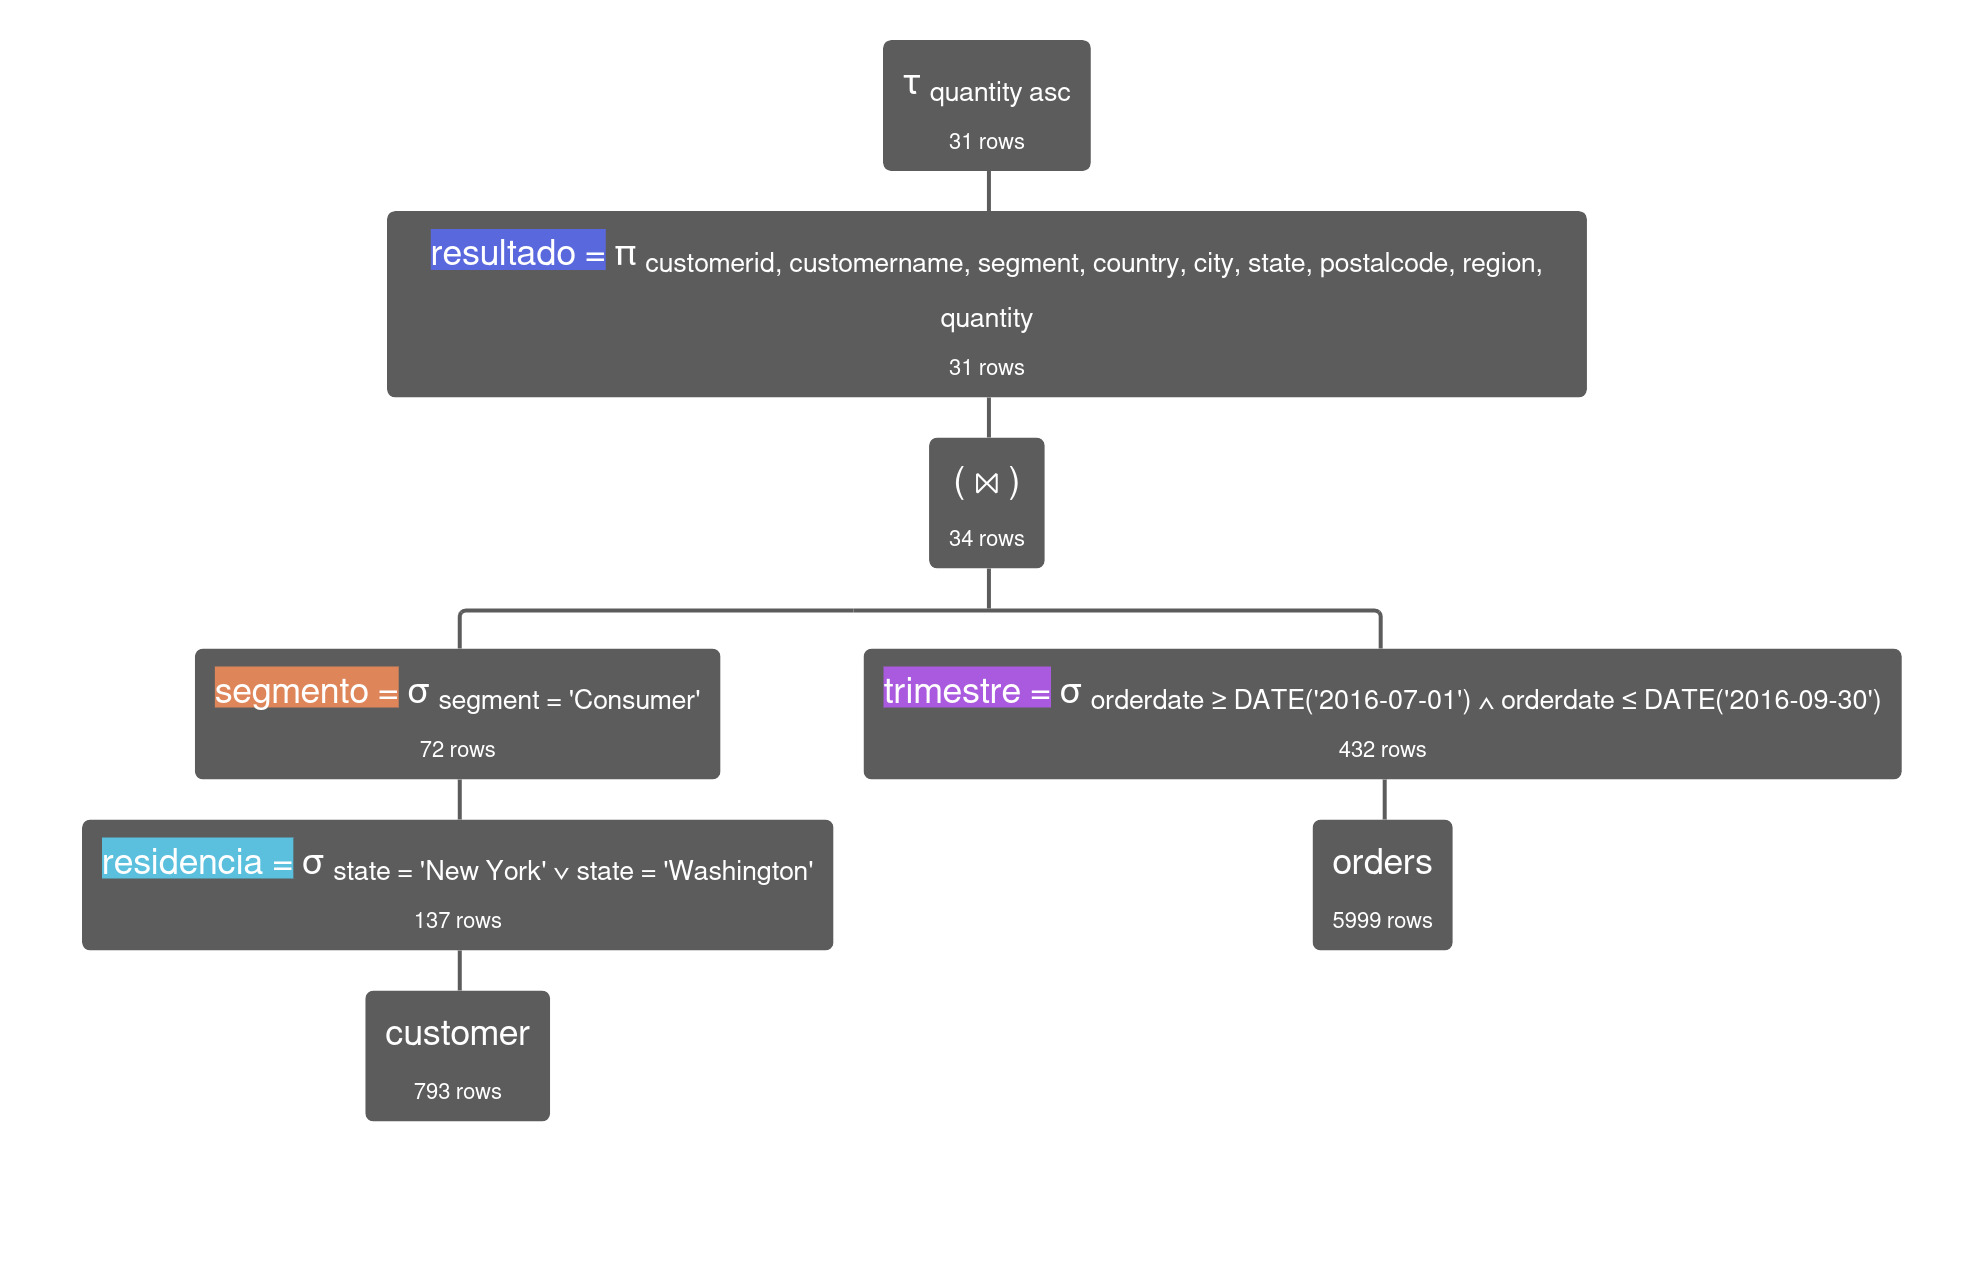
\includegraphics[width=0.7\textwidth]{figuras/2a_arbol.jpg}
\end{center}

\begin{center}
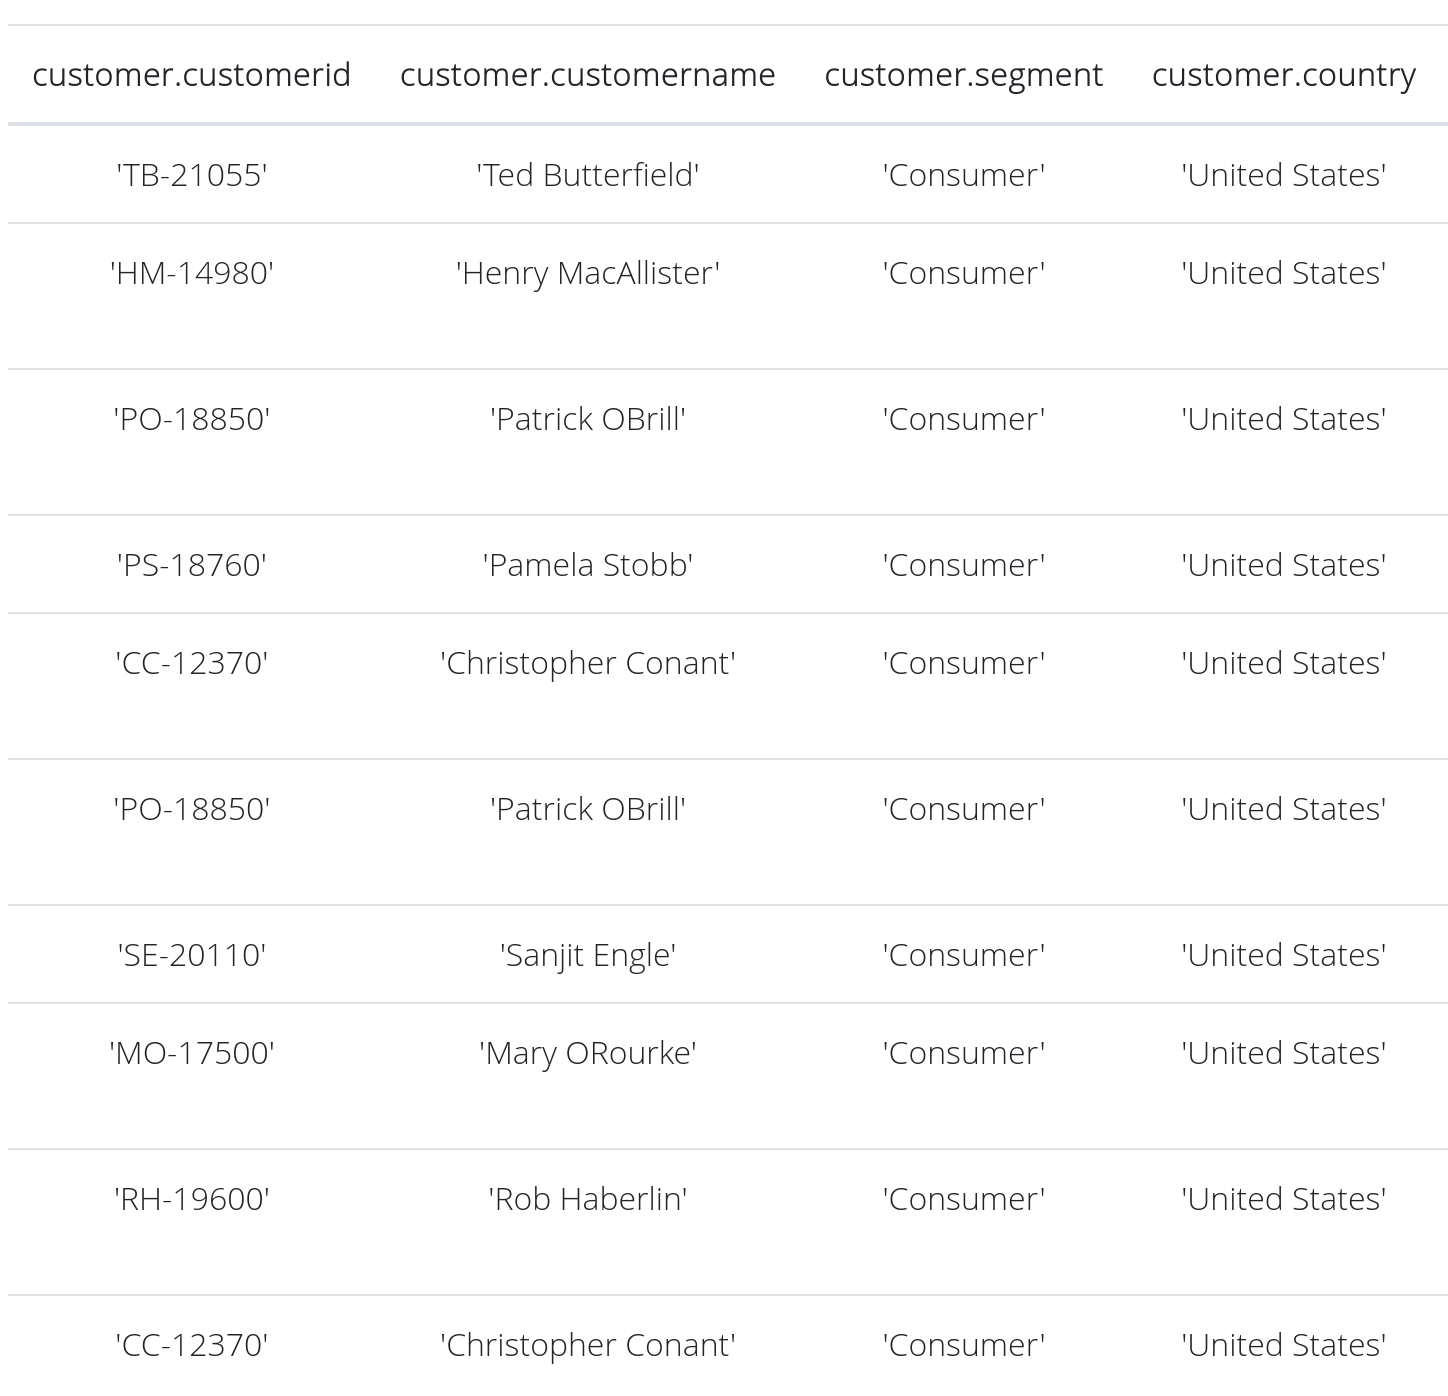
\includegraphics[width=0.38\textwidth]{figuras/2a_tuples.png}
\end{center}

\newpage

	\item Obtener una relación de los productos que pertenecen a la categoría Technology con precio mayor de \$400 y menor de \$850, pero que no hayan sido solicitados en ninguna orden.
	\item Obtener el nombre de todos los clientes que vivan en la región South y hayan solicitados productos de las subcategorías Bookcases o Chairs o Appliances o Copiers. El pedido debió de solicitarse el primer o tercer trimestre de 2015 y el modo de envío debe ser Standard Class.


	\item Toda la información de los clientes del segmento Consumer que realizaron una orden con modo de envío Second Class y que no viven en Nevada.

\begin{lstlisting}
consumidores = σ segment = 'Consumer' (customer)

pedidos = σ shipmode = 'Second Class' (orders)

clientes = σ state ≠ 'Nevada' (consumidores)

π customerid, customername, segment, country, city, state, postalcode, region
  (clientes ⨝ π customerid (pedidos))
\end{lstlisting}

\begin{center}
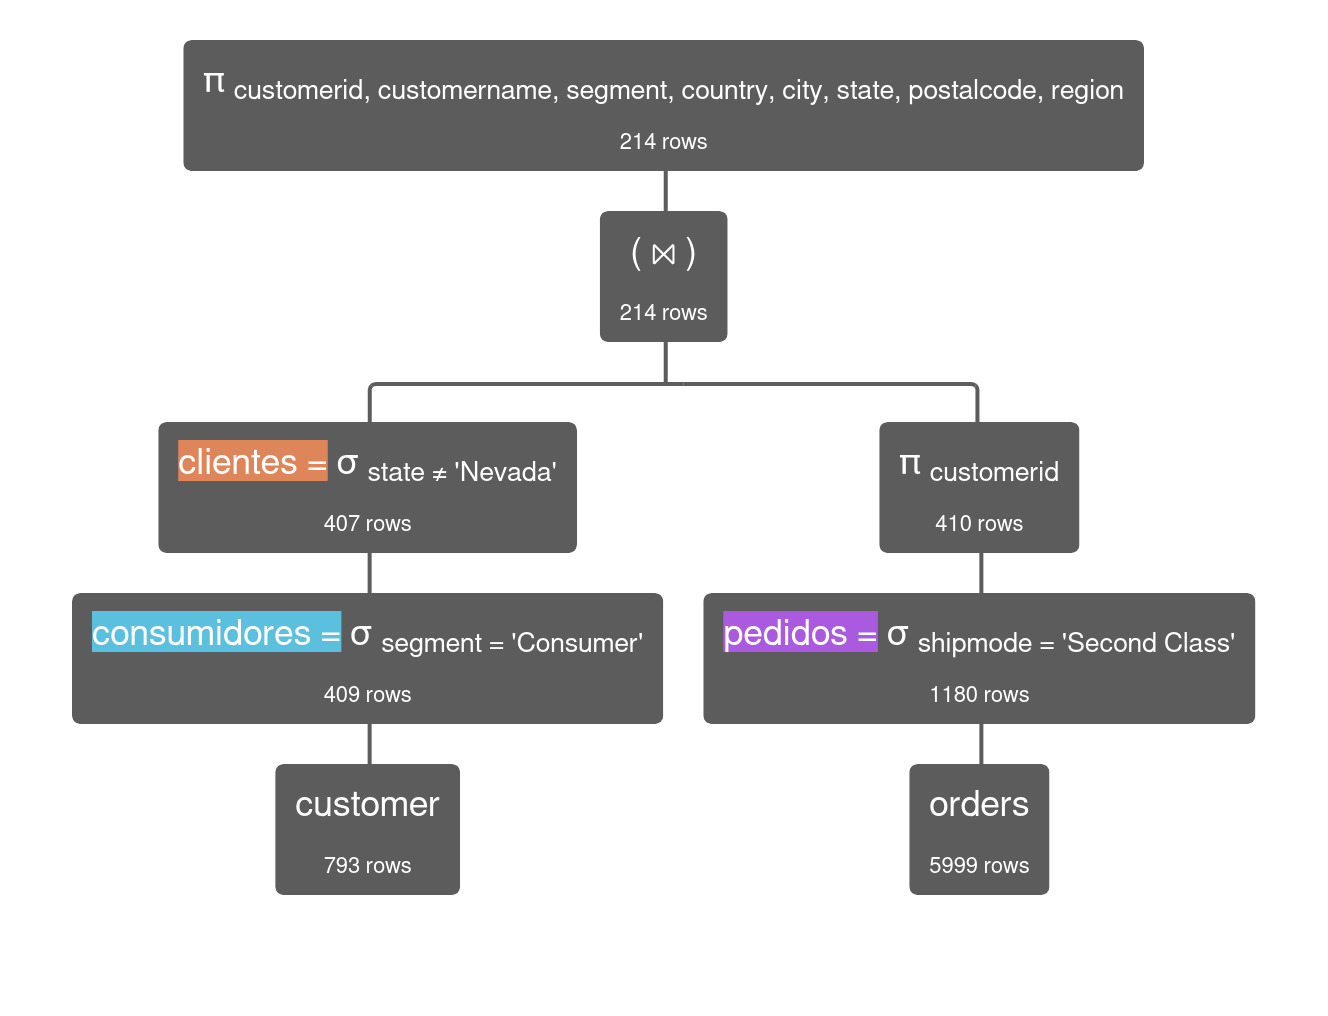
\includegraphics[width=0.75\textwidth]{figuras/2d_arbol.jpg}
\end{center}

\begin{center}
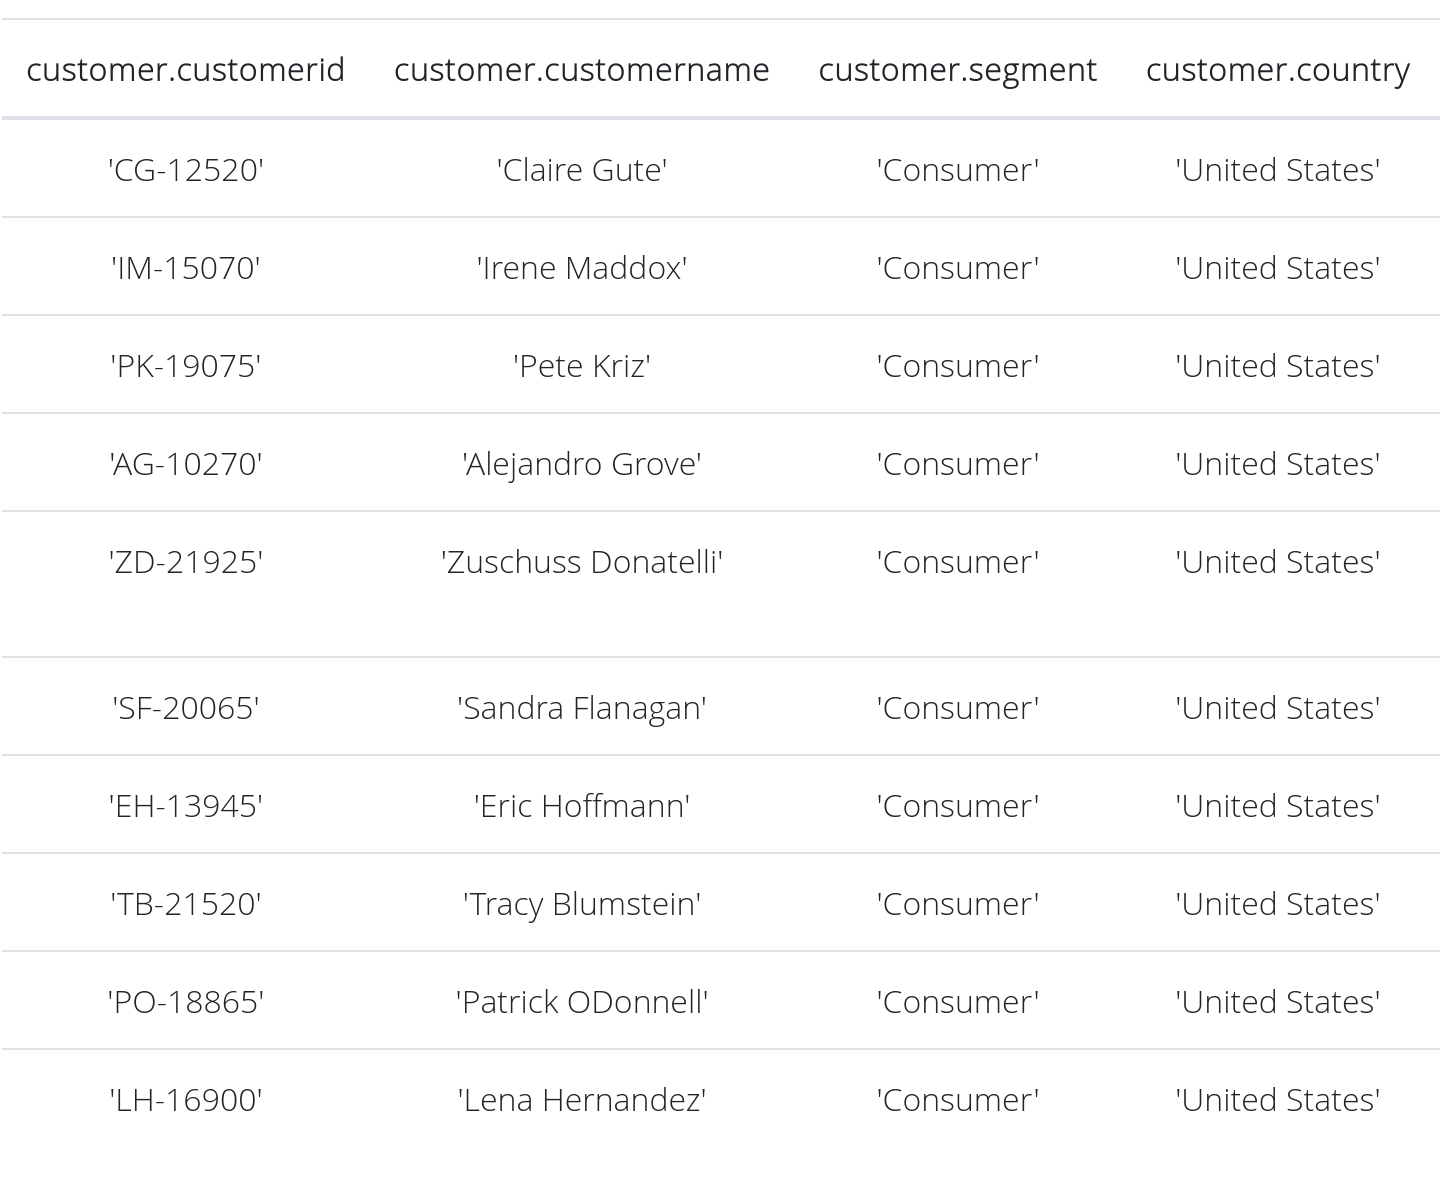
\includegraphics[width=0.4\textwidth]{figuras/2d_tuples.png}
\end{center}

\newpage

	\item Obtener el estado, segmento y el total de clientes que no han solicitado ninguna orden.
	\item Una lista que muestre la región, el estado y el total de clientes que se tienen, considerando que los clientes deben haber realizado órdenes con al menos 6 productos durante 2016 o 2017. Ordenar la información por región y estado.
	\item Obtener el modo de envío y categoría que más productos ha vendido.
	\item Una lista con la venta promedio, venta total, mayor venta, menor venta, y total de órdenes, por región, estado y ciudad. La venta promedio debe estar entre \$900 y \$1,500.

\begin{lstlisting}
detalle = customer ⨝ orders ⨝ products

importes = π region,state,city,orderid,(quantity * price) -> importe (detalle)

ventas = γ region,state,city,orderid; sum(importe)→venta (importes)

resumen = γ region,state,city; avg(venta)→promedio, sum(venta)→total, max(venta)→mayor, min(venta)→menor, count(orderid)→ordenes (ventas)

resultado = σ promedio ≥ 900 ∧ promedio ≤ 1500 (resumen)

τ region ASC,state ASC,city ASC (resultado)
\end{lstlisting}

\begin{figure}[h]
\centering
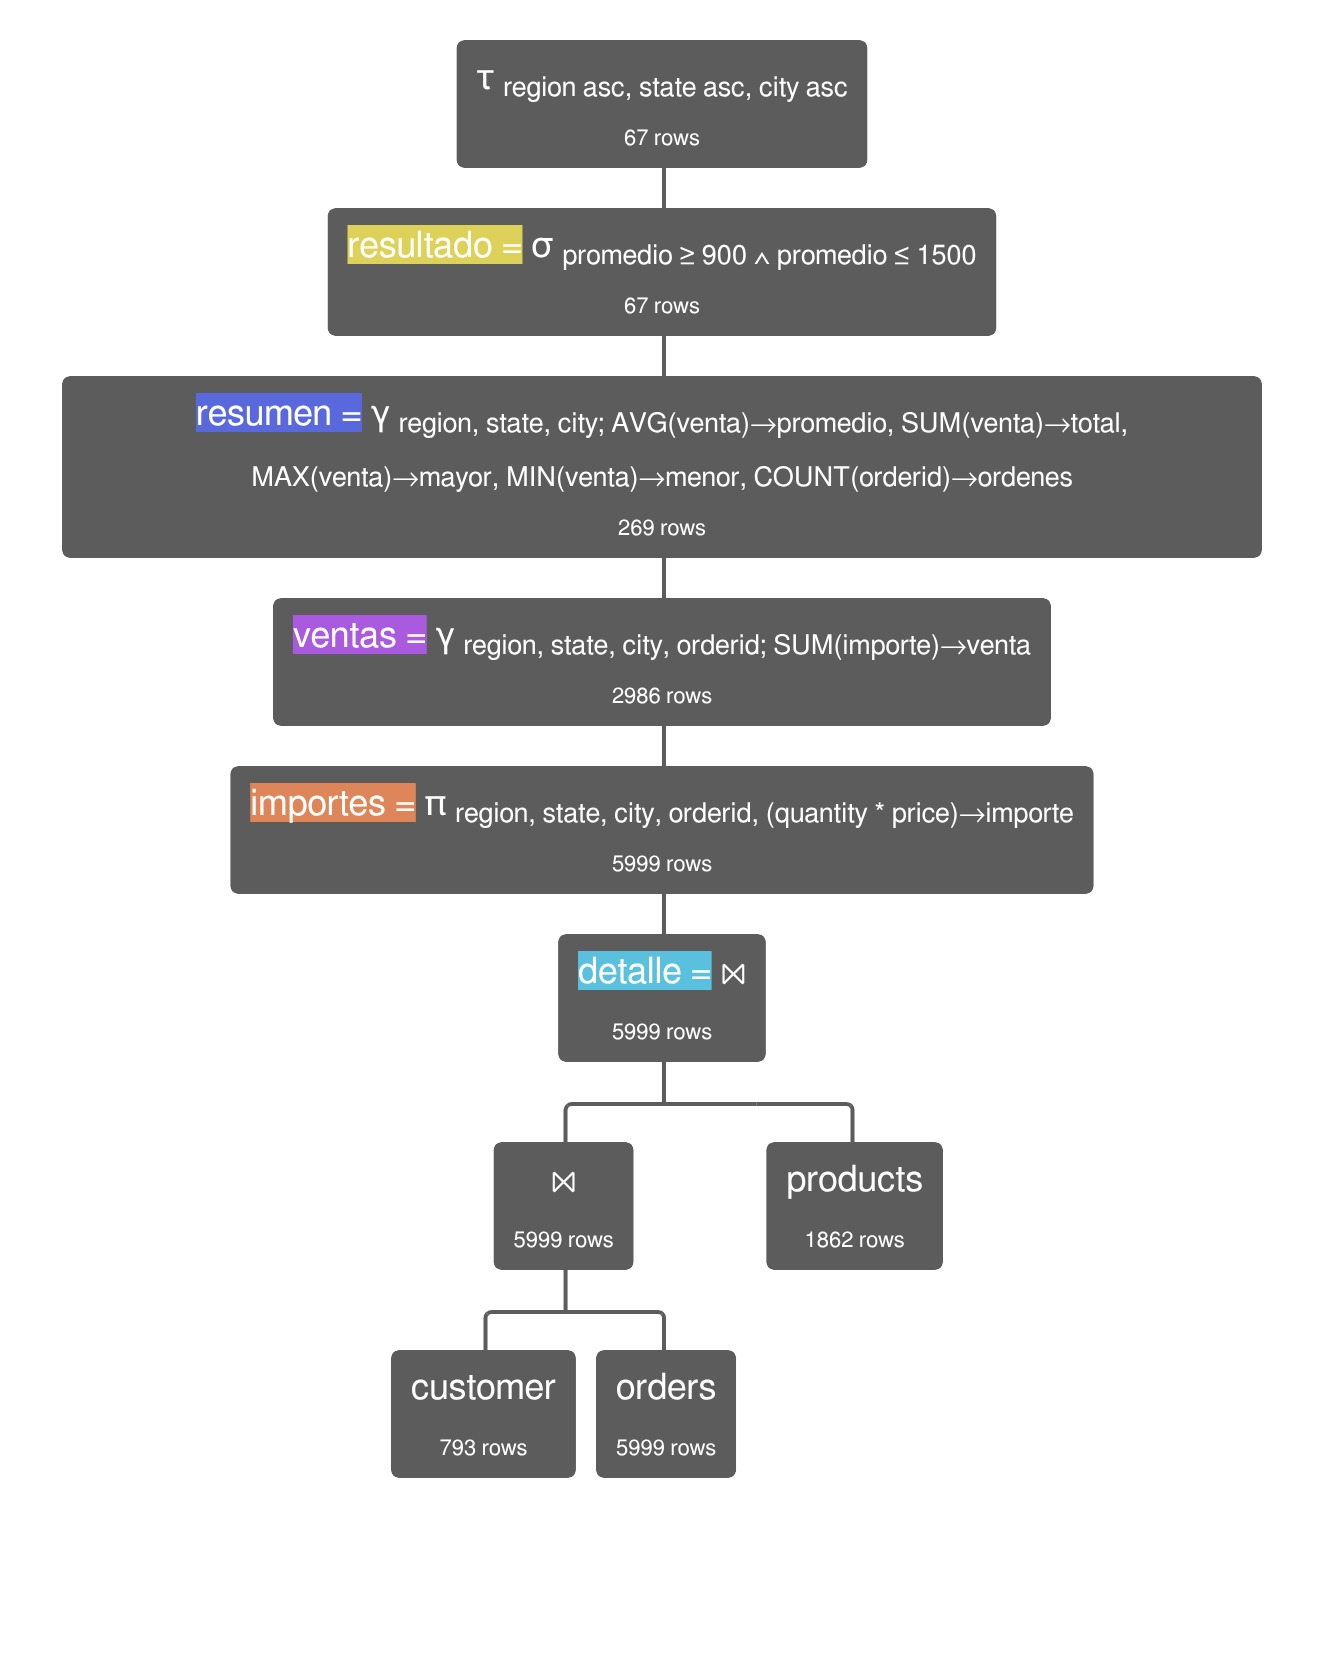
\includegraphics[width=0.5\textwidth]{figuras/2h_1.jpg}
\end{figure}

\begin{figure}[h]
\centering
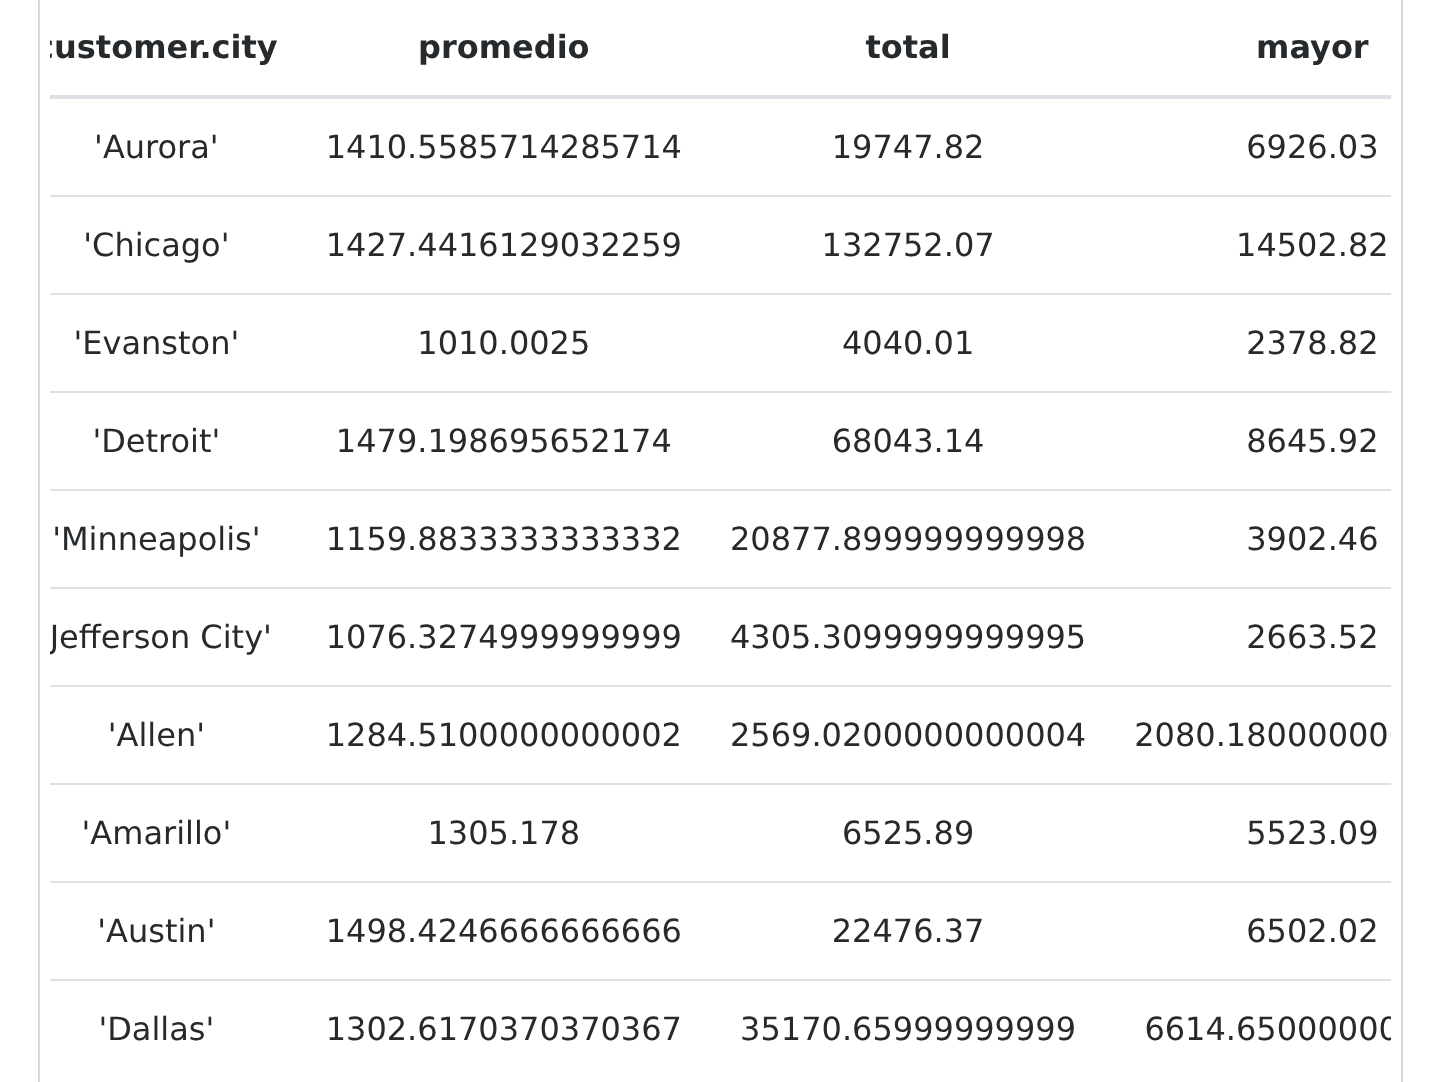
\includegraphics[width=0.3\textwidth]{figuras/2h_2.png}
\end{figure}

\newpage
	\item El estado que ha realizado la menor cantidad de órdenes. Se debe mostrar también el total de ordenes que haya entregado.

\begin{lstlisting}
ordenes = π state,orderid (customer ⨝ orders)

por_estado = γ state; count(orderid)→total (ordenes)

minimo = γ ; min(total)→menor (por_estado)

resultado = π state,total (σ total = menor (por_estado ⨯ minimo))

resultado
\end{lstlisting}

\begin{center}
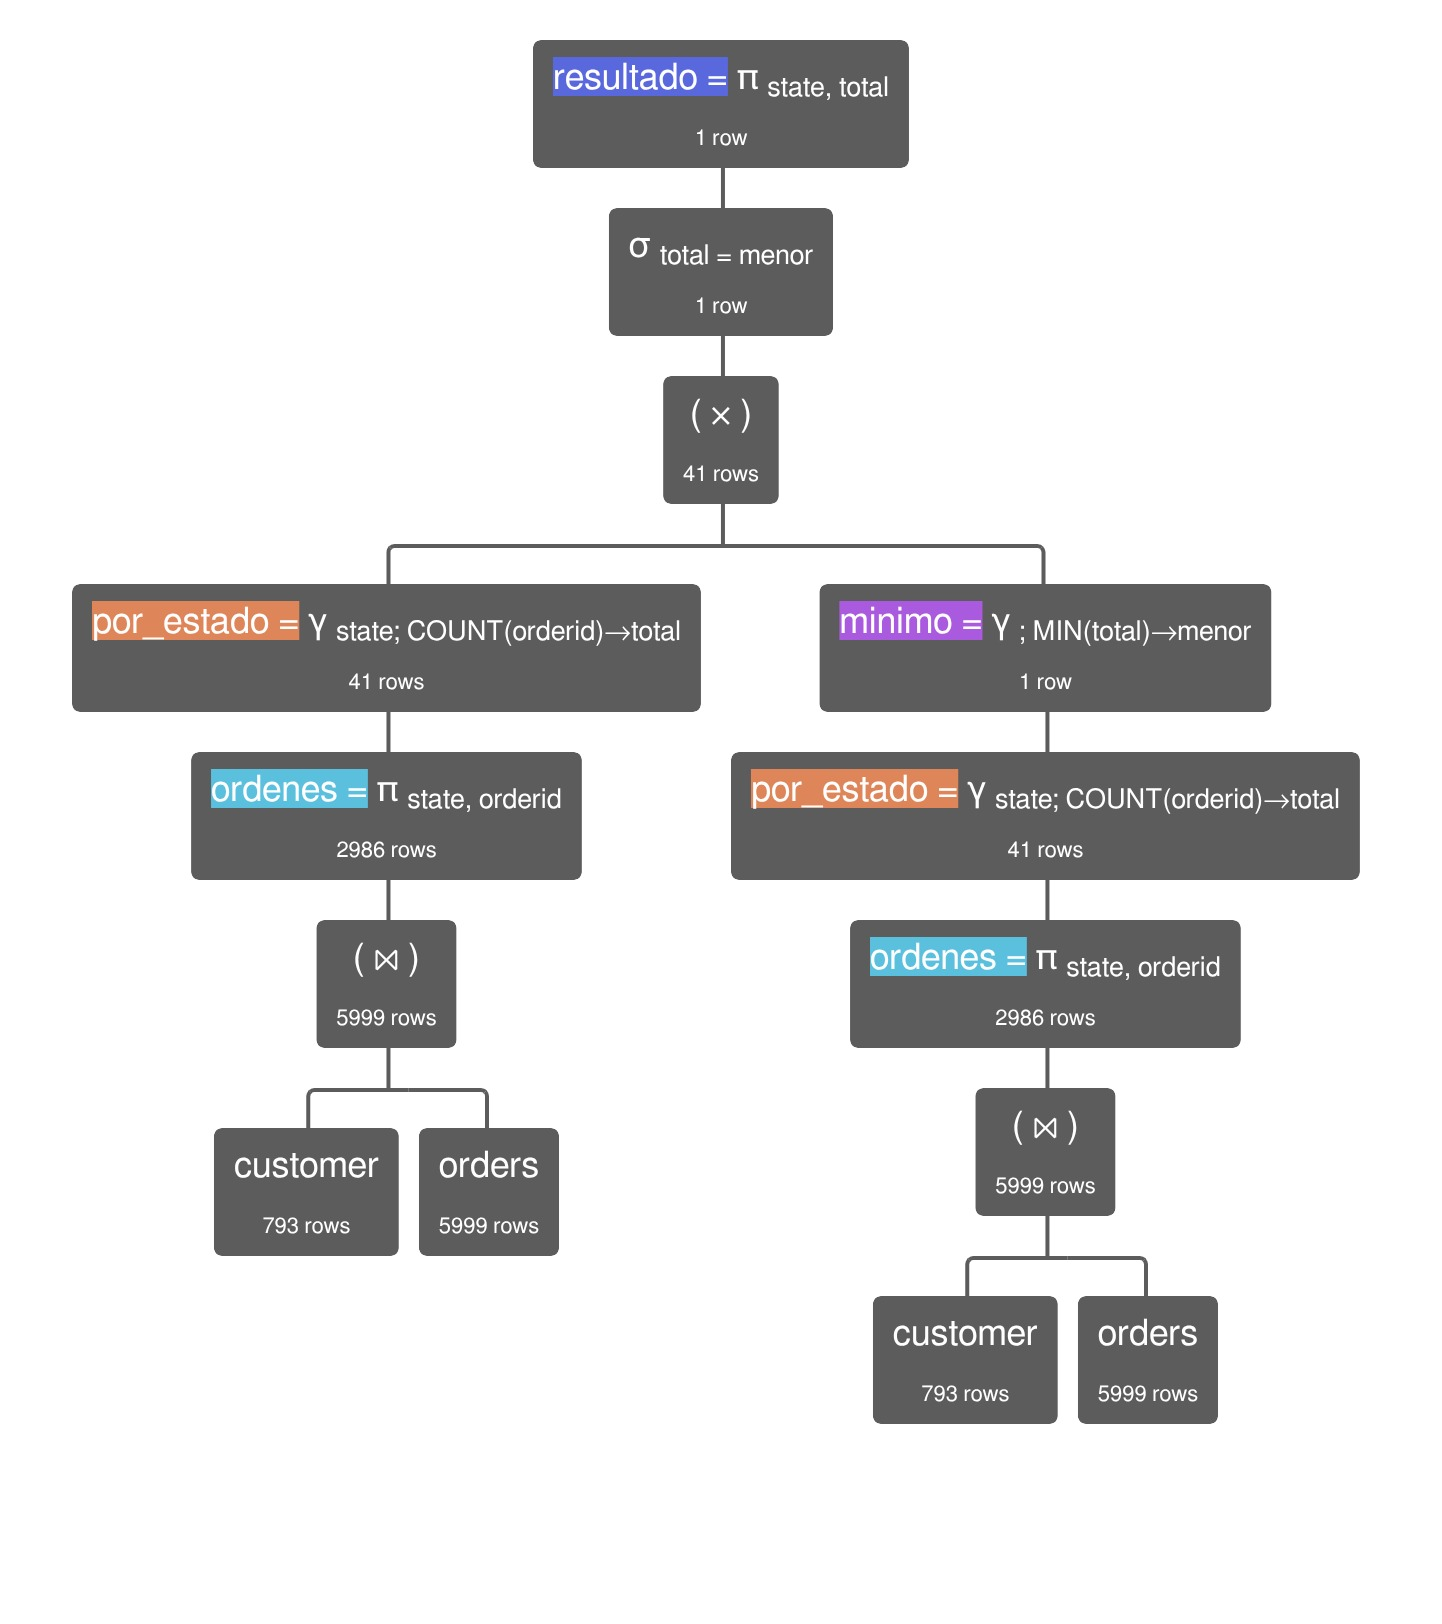
\includegraphics[width=0.65\textwidth]{figuras/2i_1.jpg}
\end{center}

\begin{center}

\includegraphics[width=0.4\textwidth]{figuras/2i_2.png}
\end{center}

\newpage

	\item La información del cliente que más órdenes haya efectuado. Mostrar el número de órdenes que ha realizado.

\begin{lstlisting}
ordenes = π customerid,orderid (orders)

por_cliente = γ customerid; count(orderid)→total (ordenes)

maximo = γ ; max(total)→mayor (por_cliente)

resultado = σ total = mayor (por_cliente ⨯ maximo)

π customerid,customername,segment,country,city,state,postalcode,region,total (customer ⨝ resultado)
\end{lstlisting}

\begin{center}
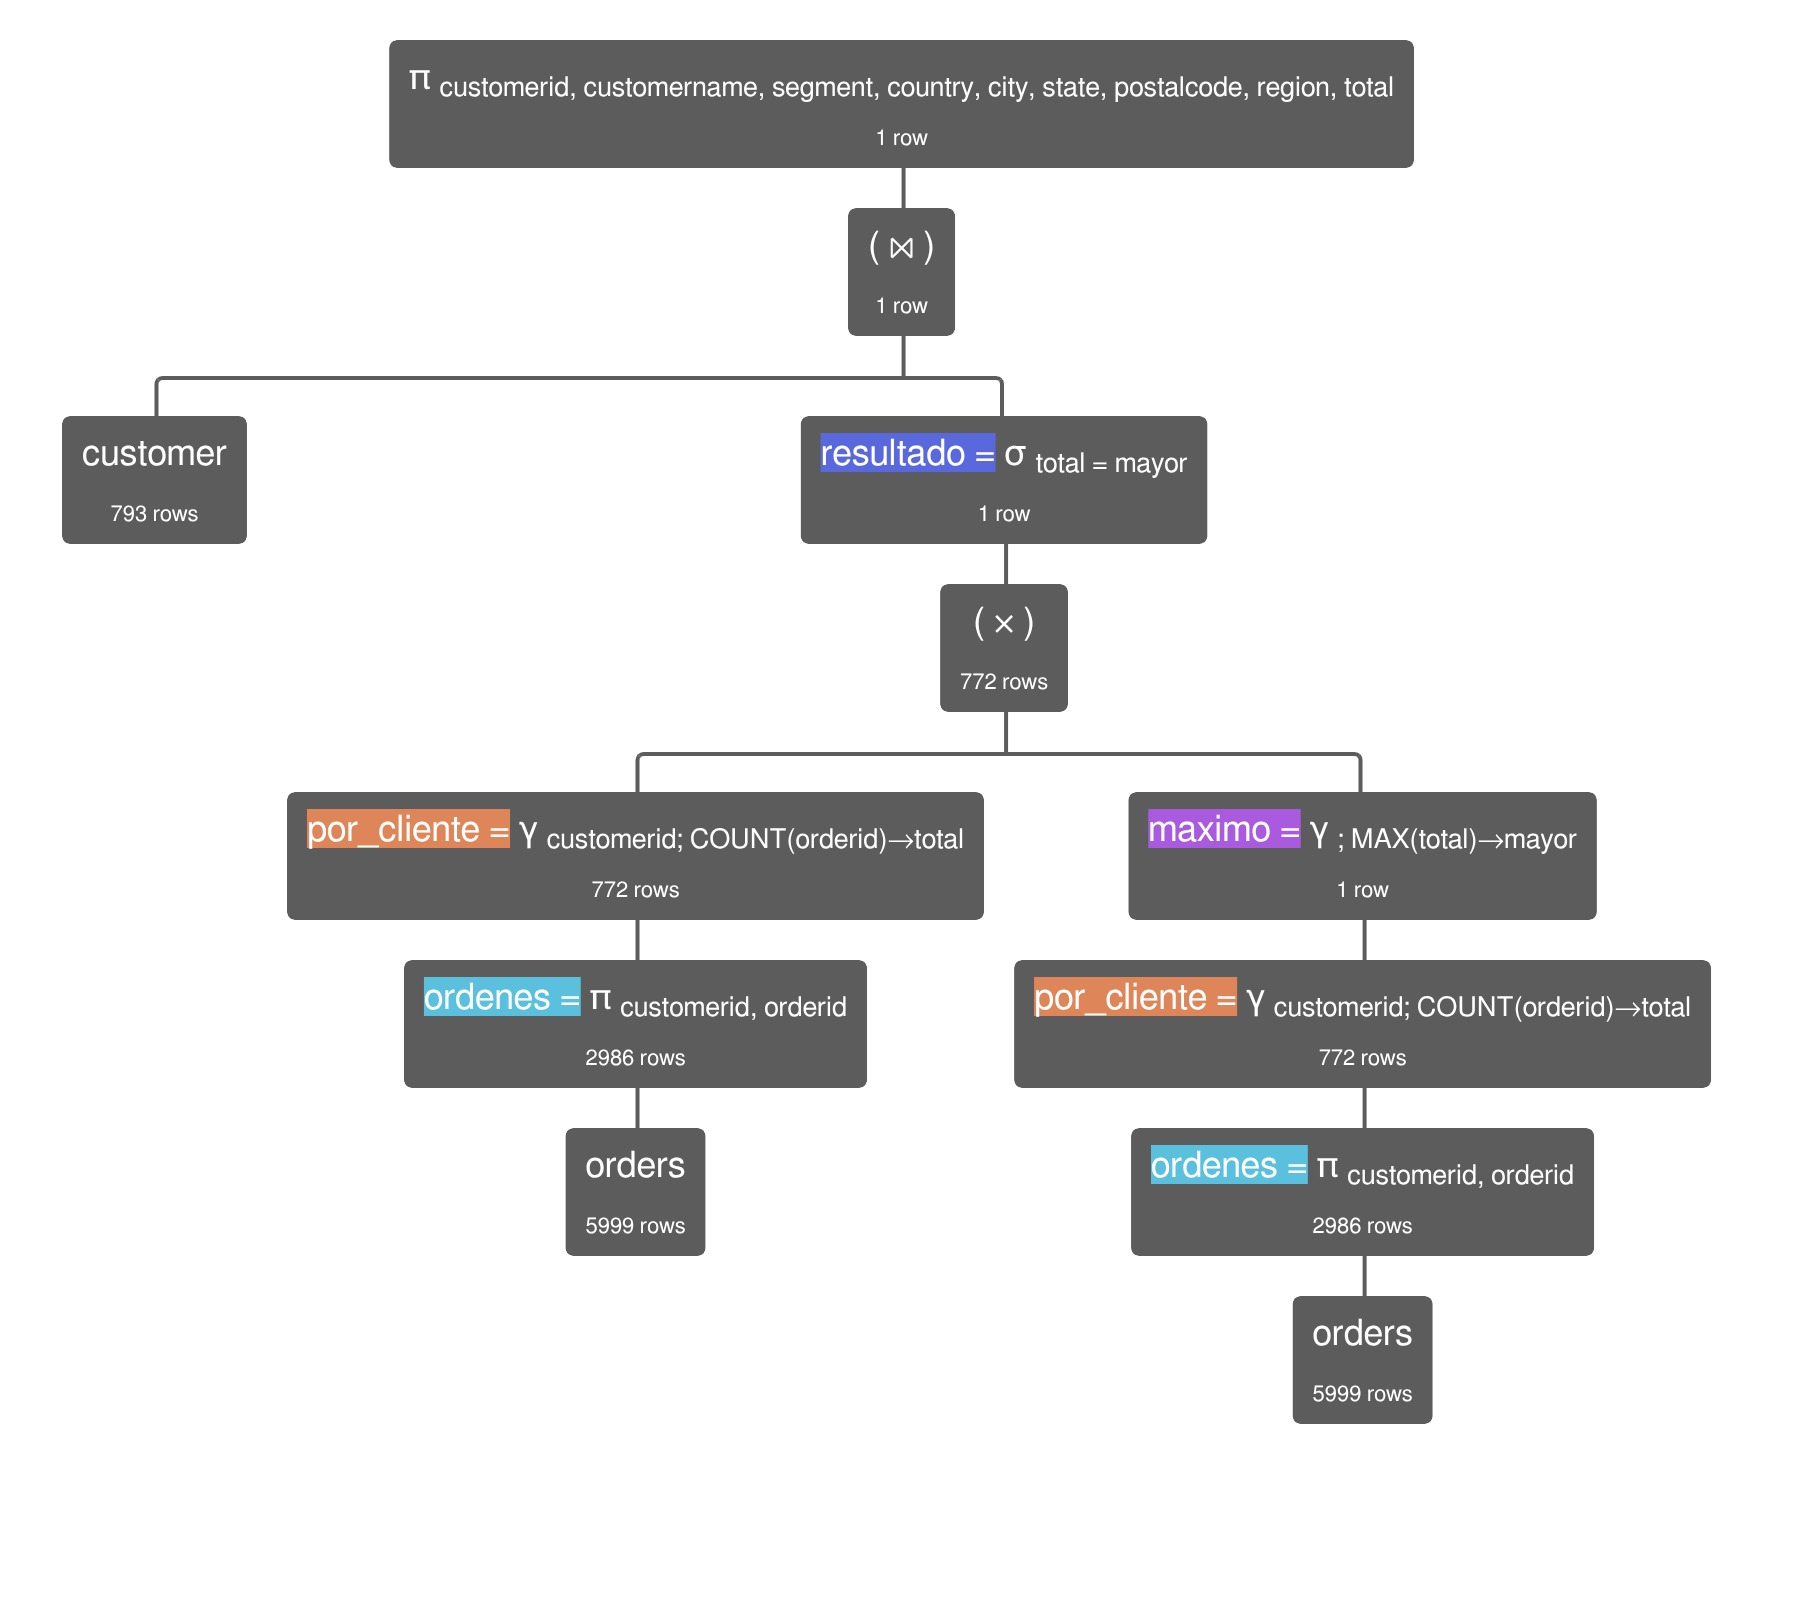
\includegraphics[width=0.75\textwidth]{figuras/2j_1.jpg}
\end{center}

\begin{center}

\includegraphics[width=0.4\textwidth]{figuras/2j_2.png}
\end{center}

\newpage

\end{enumerate}


\subsection*{Operaciones de mantenimiento de datos: borrado, inserción y actualización}


\begin{enumerate}[label=\alph*., leftmargin=*]
	\item Borrar toda la información del cliente \textbf{Paul Stevenson}.

\begin{lstlisting}
orders = orders − π orderid, orderdate, shipdate, shipmode, customerid, productid, quantity
         (σ customername = 'Paul Stevenson' (customer ⨝= orders))

customer = customer − σ customername = 'Paul Stevenson' (customer)
\end{lstlisting}

Paul Stevenson (PS-18970) tiene 6 renglones de orden en 5 órdenes.
Se eliminan primero sus órdenes y después su registro en \texttt{customer}
para respetar la llave foránea. En Relax, la verificación se hace con
\texttt{orders\_sin\_paul} y \texttt{customer\_sin\_paul}; el join externo
derecho se escribe \texttt{right join}.

% ==========================================
% Página de mayor tamaño para los árboles y las tuplas
% (misma técnica que la Práctica 05)
% ==========================================
\clearpage
\pdfpagewidth=35cm
\pdfpageheight=32cm
\setlength{\textwidth}{34cm}
\setlength{\hsize}{34cm}
\setlength{\oddsidemargin}{\dimexpr(\pdfpagewidth-\textwidth)/2 - 1in\relax}
\setlength{\evensidemargin}{\oddsidemargin}
\setlength{\textheight}{31cm}
\setlength{\vsize}{31cm}
\setlength{\headheight}{0pt}
\setlength{\headsep}{0pt}
\setlength{\topmargin}{\dimexpr(\pdfpageheight-\textheight)/2 - 1in\relax}
\thispagestyle{empty}
\vspace*{0.2cm}
\centering
\begin{tabular}{@{}c@{\hspace{0.5cm}}c@{}}
\begin{minipage}[t]{0.42\textwidth}
  \centering
  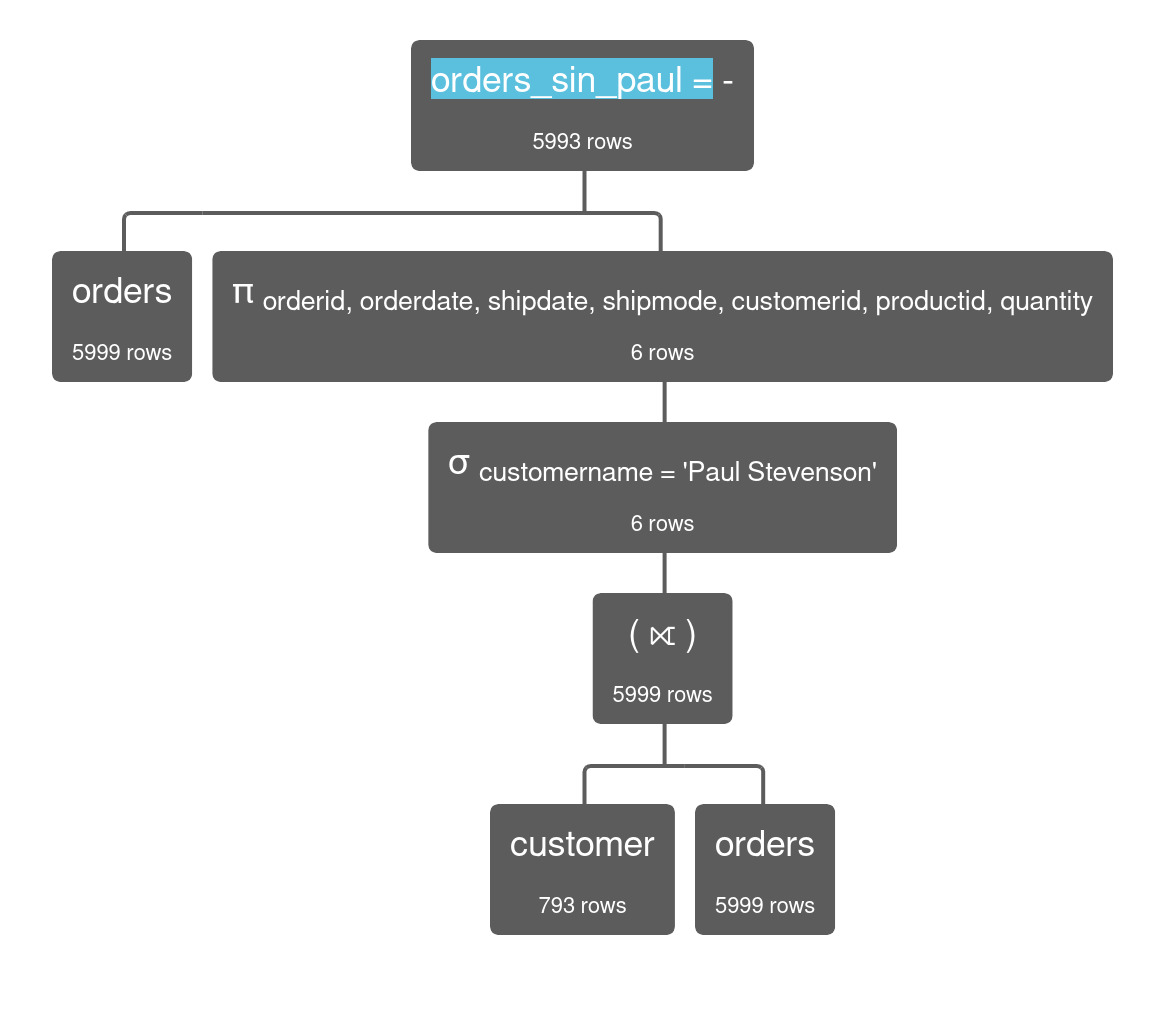
\includegraphics[width=\linewidth]{figuras/3a_arbol.jpg}\\[0.1cm]
  {\small Árbol de \texttt{orders\_sin\_paul}}
\end{minipage} &
\begin{minipage}[t]{0.42\textwidth}
  \centering
  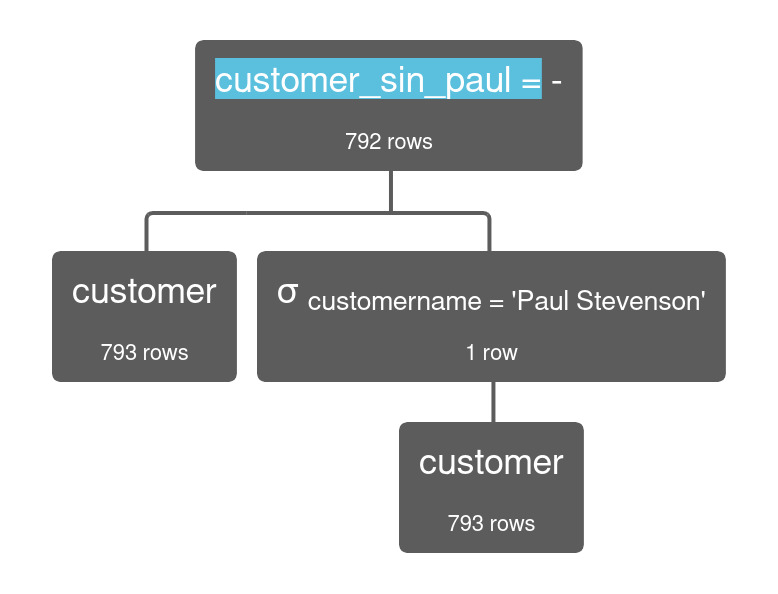
\includegraphics[width=\linewidth]{figuras/3a_arbol_customer.jpg}\\[0.1cm]
  {\small Árbol de \texttt{customer\_sin\_paul}}
\end{minipage}
\end{tabular}

\vspace{0.35cm}
\begin{tabular}{@{}c@{\hspace{0.5cm}}c@{}}
\begin{minipage}[t]{0.42\textwidth}
  \centering
  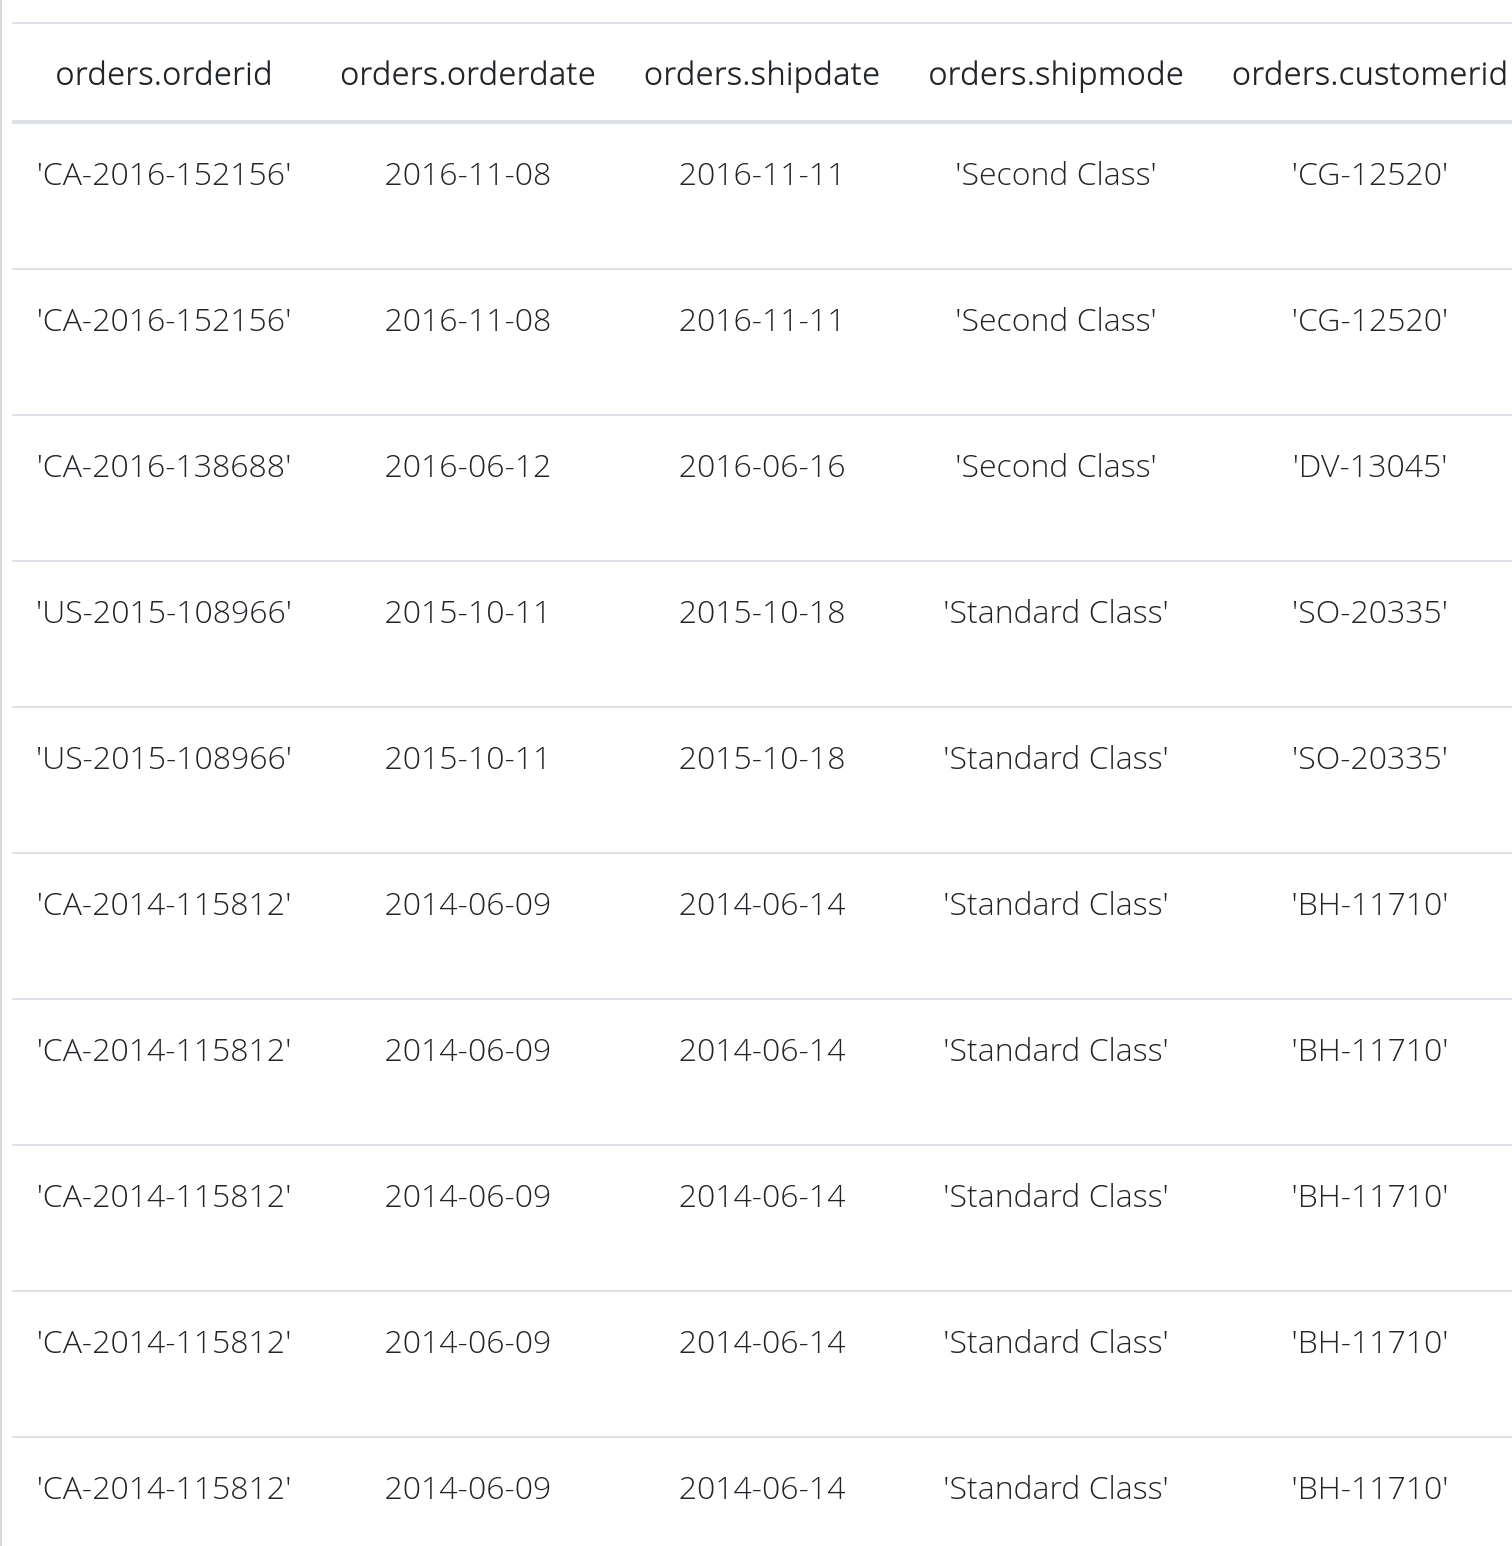
\includegraphics[width=\linewidth]{figuras/3a_tuplas.png}\\[0.1cm]
  {\small Primeros renglones de \texttt{orders\_sin\_paul}}
\end{minipage} &
\begin{minipage}[t]{0.42\textwidth}
  \centering
  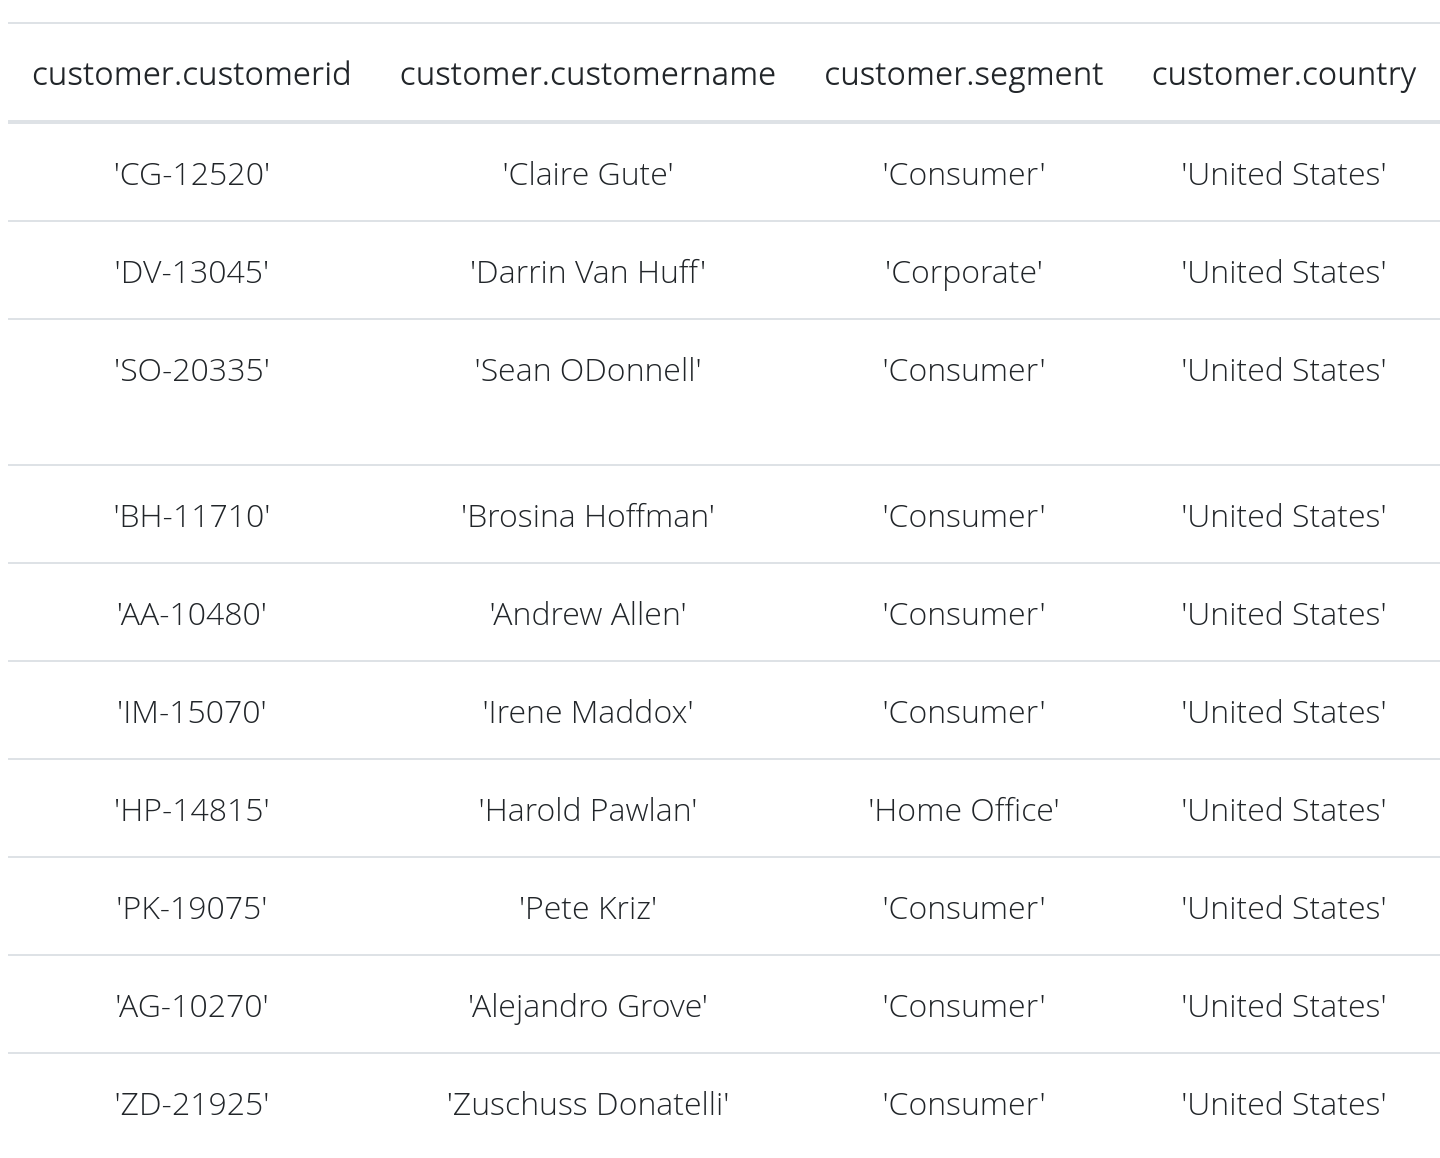
\includegraphics[width=\linewidth]{figuras/3a_tuplas_customer.png}\\[0.1cm]
  {\small Primeros renglones de \texttt{customer\_sin\_paul}}
\end{minipage}
\end{tabular}

\vspace{0.3cm}
{\small Las tuplas mostradas son los primeros renglones de las relaciones
resultantes; Paul Stevenson ya no aparece en \texttt{orders\_sin\_paul}
ni en \texttt{customer\_sin\_paul}.}
\clearpage
\restoregeometry
\pdfpagewidth=\paperwidth
\pdfpageheight=\paperheight

	\clearpage
\pdfpagewidth=35cm
\pdfpageheight=25cm
\setlength{\textwidth}{34cm}
\setlength{\hsize}{34cm}
\setlength{\oddsidemargin}{\dimexpr(\pdfpagewidth-\textwidth)/2 - 1in\relax}
\setlength{\evensidemargin}{\oddsidemargin}
\setlength{\textheight}{24cm}
\setlength{\vsize}{24cm}
\setlength{\headheight}{0pt}
\setlength{\headsep}{0pt}
\setlength{\topmargin}{\dimexpr(\pdfpageheight-\textheight)/2 - 1in\relax}
\thispagestyle{empty}
\vspace*{0.2cm}
\item Borrar todas las órdenes de la ciudad \textbf{Utah} que tengan artículos de la subcategoría \textbf{Tables}.

\begin{lstlisting}
utah_tables = π orderid (σ state = 'Utah' (customer)
                         ⨝ orders
                         ⨝ σ subcategory = 'Tables' (products))

orders = orders − (orders ⨝ utah_tables)
\end{lstlisting}

La única orden que cumple es \texttt{CA-2015-106320}, que tiene un solo renglón, por lo
que \texttt{orders\_sin\_utah} termina con 5998 renglones.

\vspace{0.35cm}
\centering
\begin{tabular}{@{}c@{\hspace{0.6cm}}c@{}}
	\begin{minipage}[t]{0.38\textwidth}
		\centering
		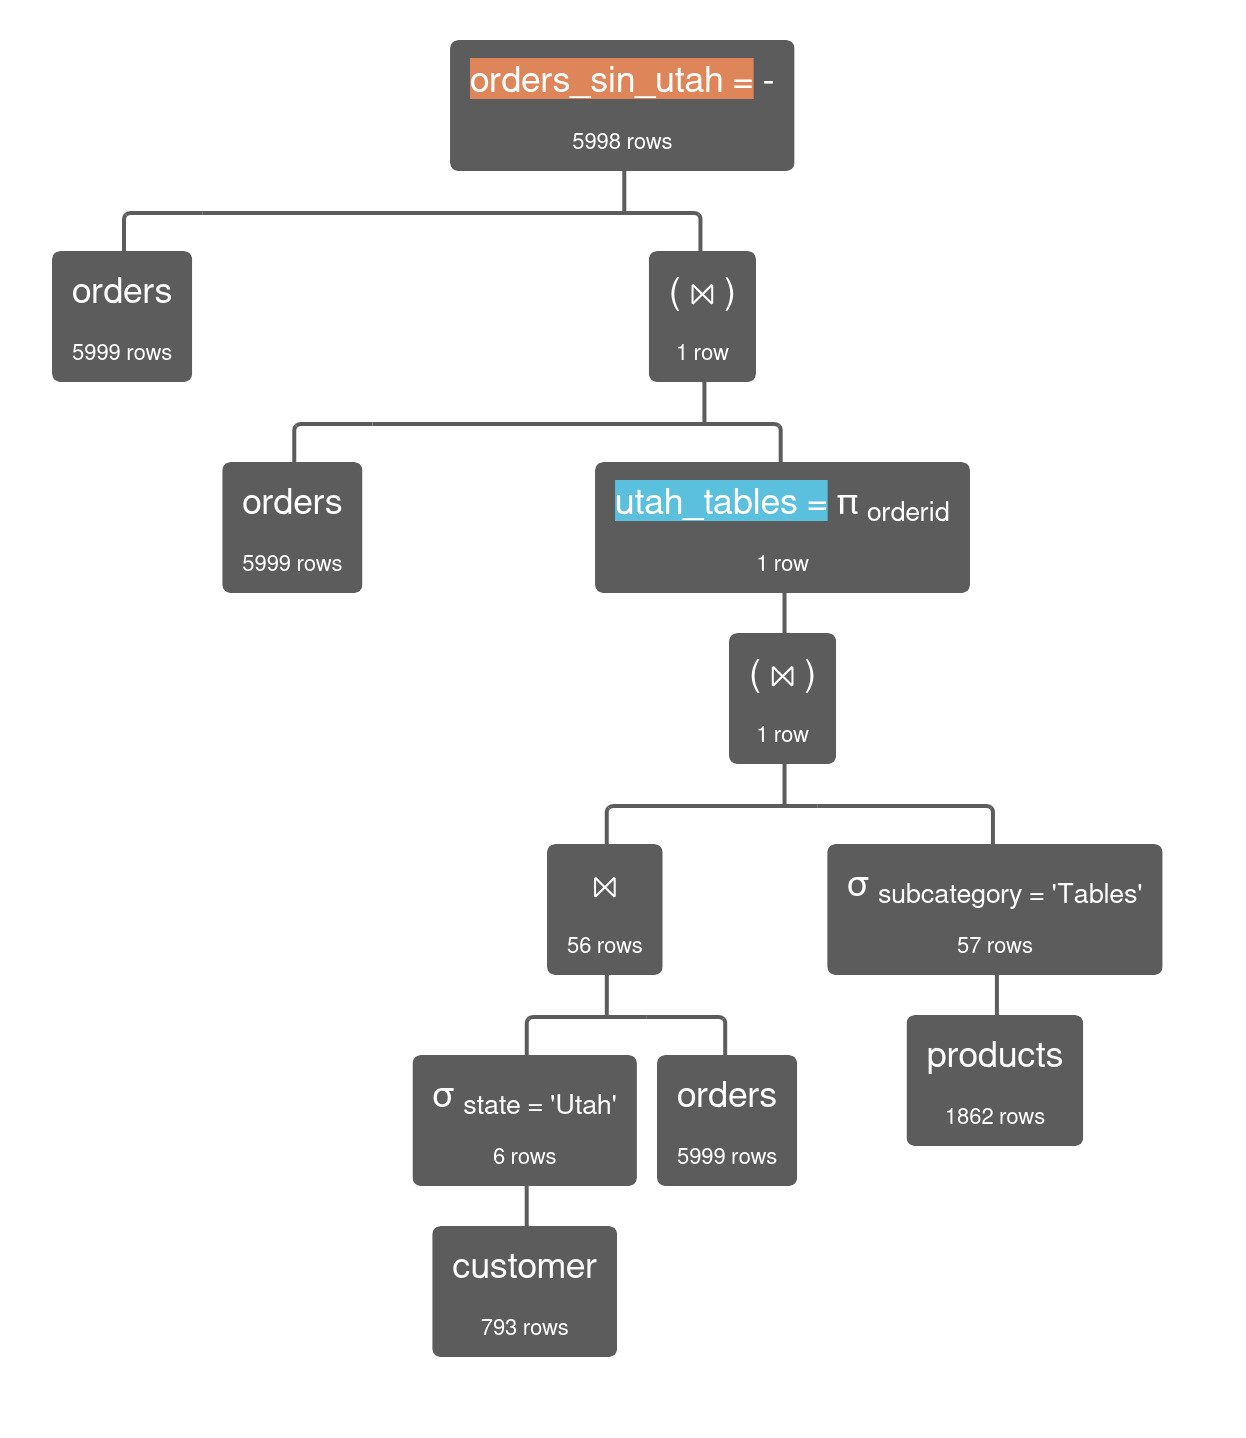
\includegraphics[width=\linewidth]{figuras/3b_arbol.jpg}\\[0.1cm]
		{\small Árbol de \texttt{orders\_sin\_utah}}
	\end{minipage} &
	\begin{minipage}[t]{0.38\textwidth}
		\centering
		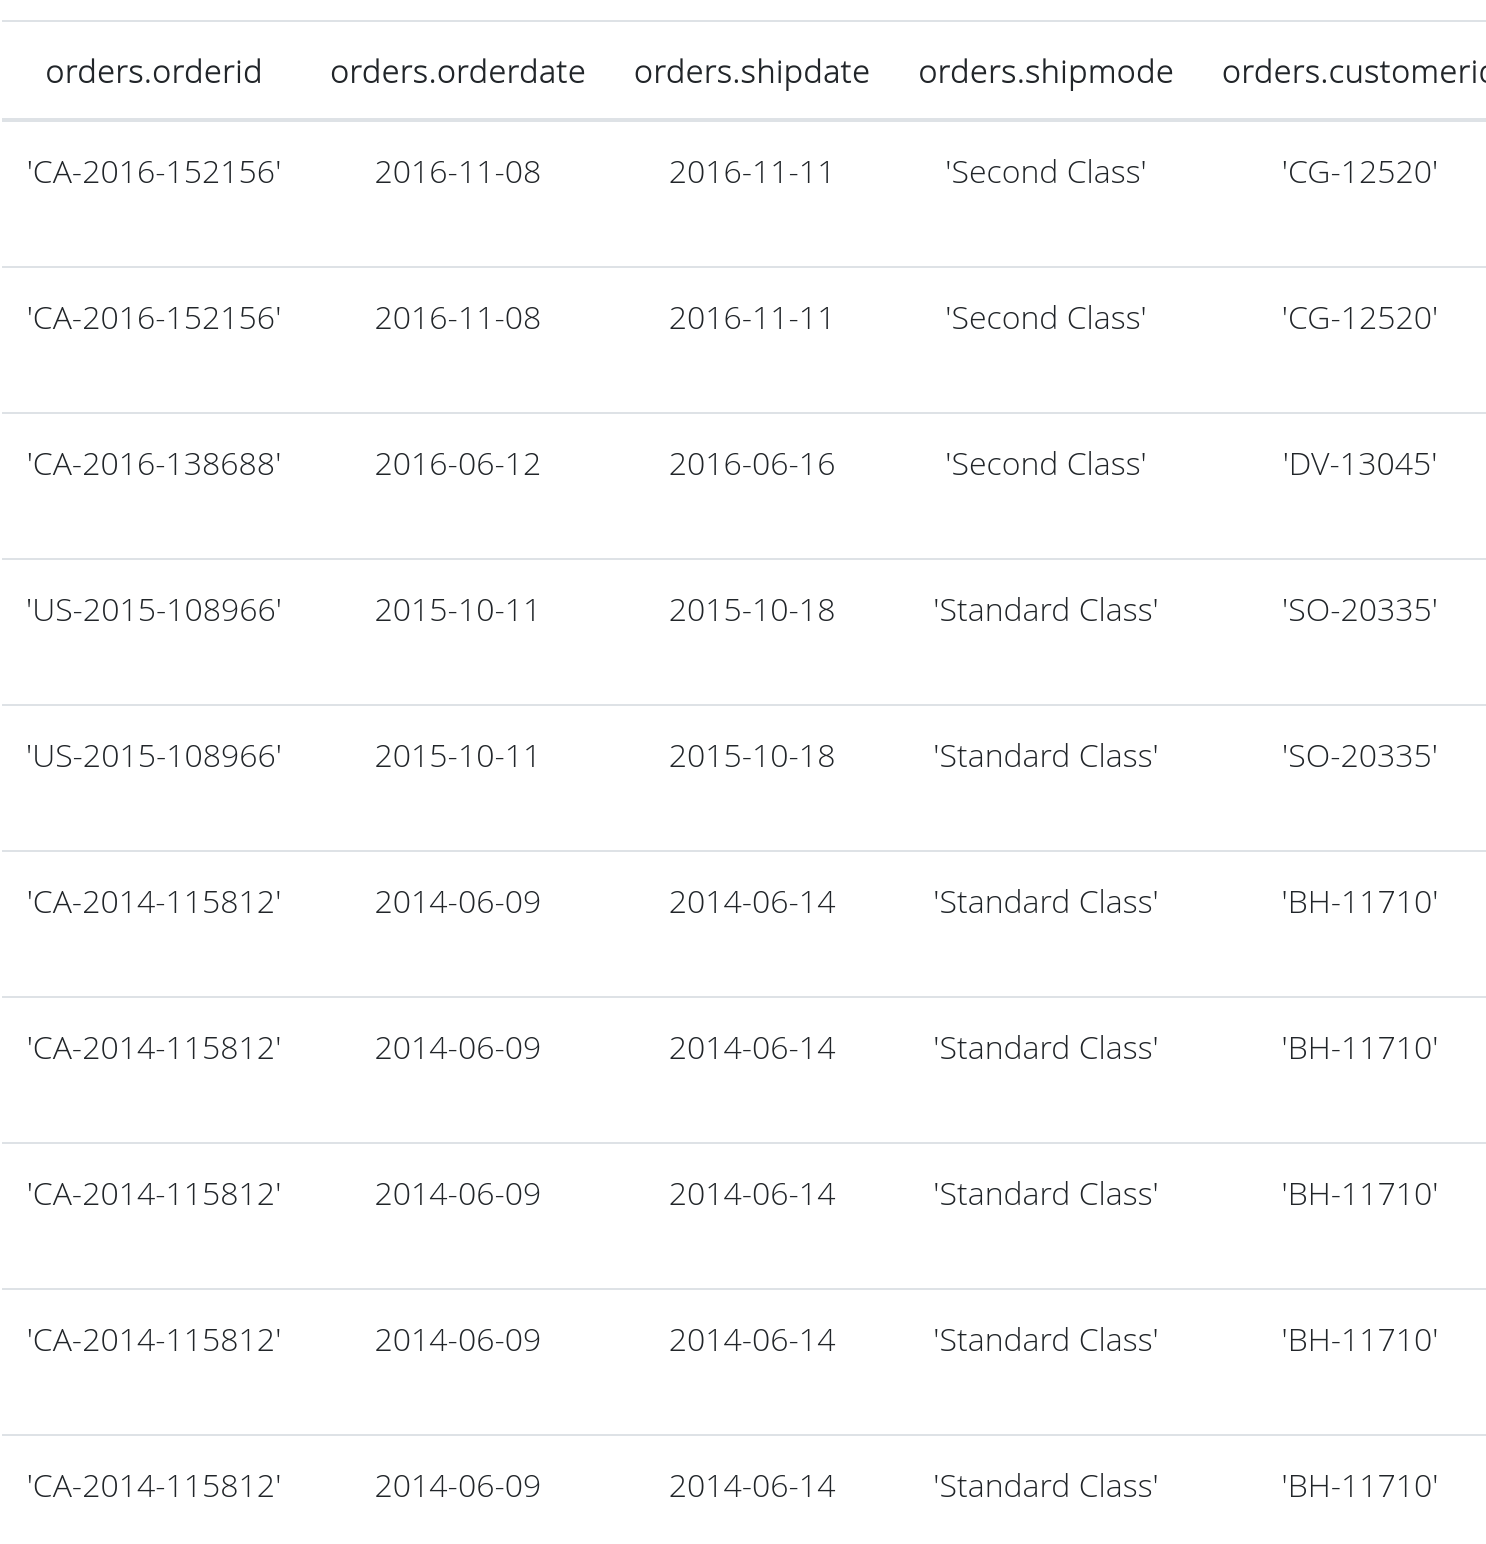
\includegraphics[width=\linewidth]{figuras/3b_tuplas.png}\\[0.1cm]
		{\small Primeros renglones de \texttt{orders\_sin\_utah}}
	\end{minipage}
\end{tabular}

\vspace{0.3cm}
{\small Las tuplas mostradas son los primeros renglones de la relación
	resultante; la orden \texttt{CA-2015-106320} ya no aparece.}
\clearpage
\restoregeometry
\pdfpagewidth=\paperwidth
\pdfpageheight=\paperheight

	\item La clienta \textbf{Lena Cacioppo} compró un producto de cada subcategoría de \textbf{Furniture}. Deberás elegir los productos que desees e indicar como parte de esta consulta, la información que se agregará en cada caso.

\begin{lstlisting}
lena_customerid = π customerid (σ customername = 'Lena Cacioppo' (customer))
furniture_types = π subcategory (σ category = 'Furniture' (products))
lena_orders = {
  orderid:string, orderdate:date, shipdate:date, shipmode:string, customerid:string, productid:string, quantity:number
  'US-2026-342349', 2026-10-26, 2026-10-30, 'Same Day', 'LC-16870', 'FUR-BO-10001798', 1
	'US-2026-342349', 2026-10-26, 2026-10-30, 'Same Day', 'LC-16870', 'FUR-CH-10000454', 1
	'US-2026-342349', 2026-10-26, 2026-10-30, 'Same Day', 'LC-16870', 'FUR-TA-10000577', 1
	'US-2026-342349', 2026-10-26, 2026-10-30, 'Same Day', 'LC-16870', 'FUR-FU-10001487', 1
}

orders U lena_orders
\end{lstlisting}

\begin{center}
  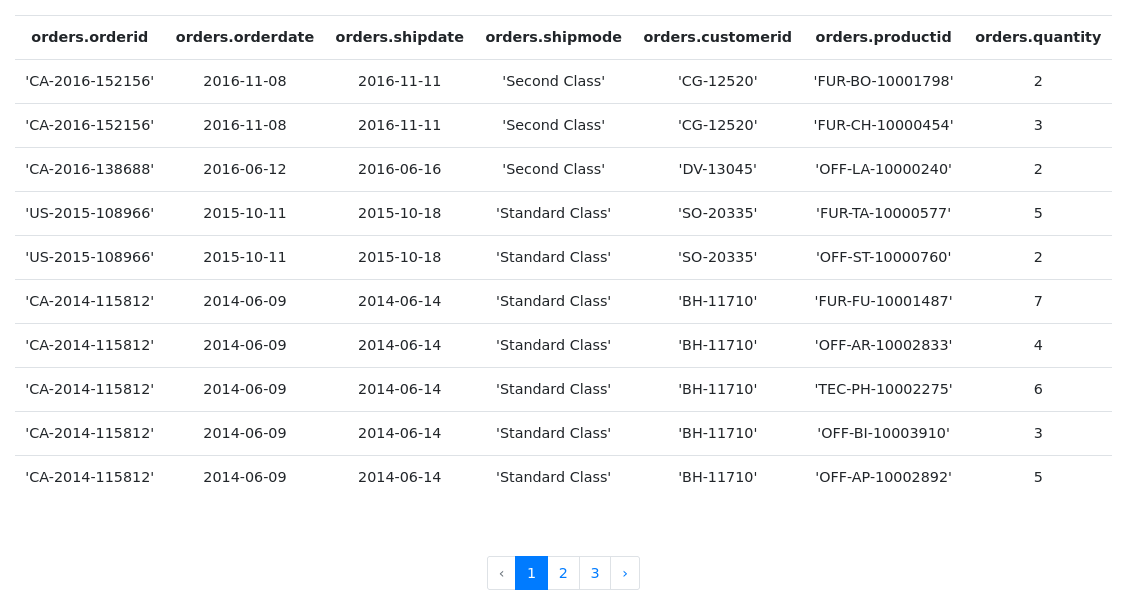
\includegraphics[width=0.7\textwidth]{figuras/3c_1.png}
\end{center}

\begin{center}
  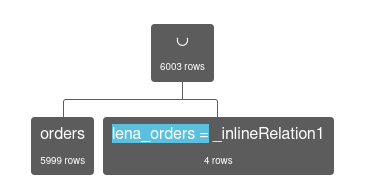
\includegraphics[width=0.7\textwidth]{figuras/3c_2.png}
\end{center}

	% \newpage
\item Aumentar los precios de los productos de la subcategoría \textbf{Phones} en un 8\%.

\begin{lstlisting}
phones = σ subcategory = 'Phones' (products)

products = (products − phones)
         ∪ π productid, category, subcategory, price * 1.08 → price (phones)
\end{lstlisting}

Se actualizan los 184 productos de la subcategoría \texttt{Phones};
la relación \texttt{products} conserva sus 1862 renglones.
Las tuplas mostradas corresponden a los teléfonos ya actualizados
(\texttt{Phones}); se muestran por separado porque en la tabla general
de \texttt{products} los registros de \texttt{Phones} son muy escasos
(184 de 1862 renglones).

\begin{center}
  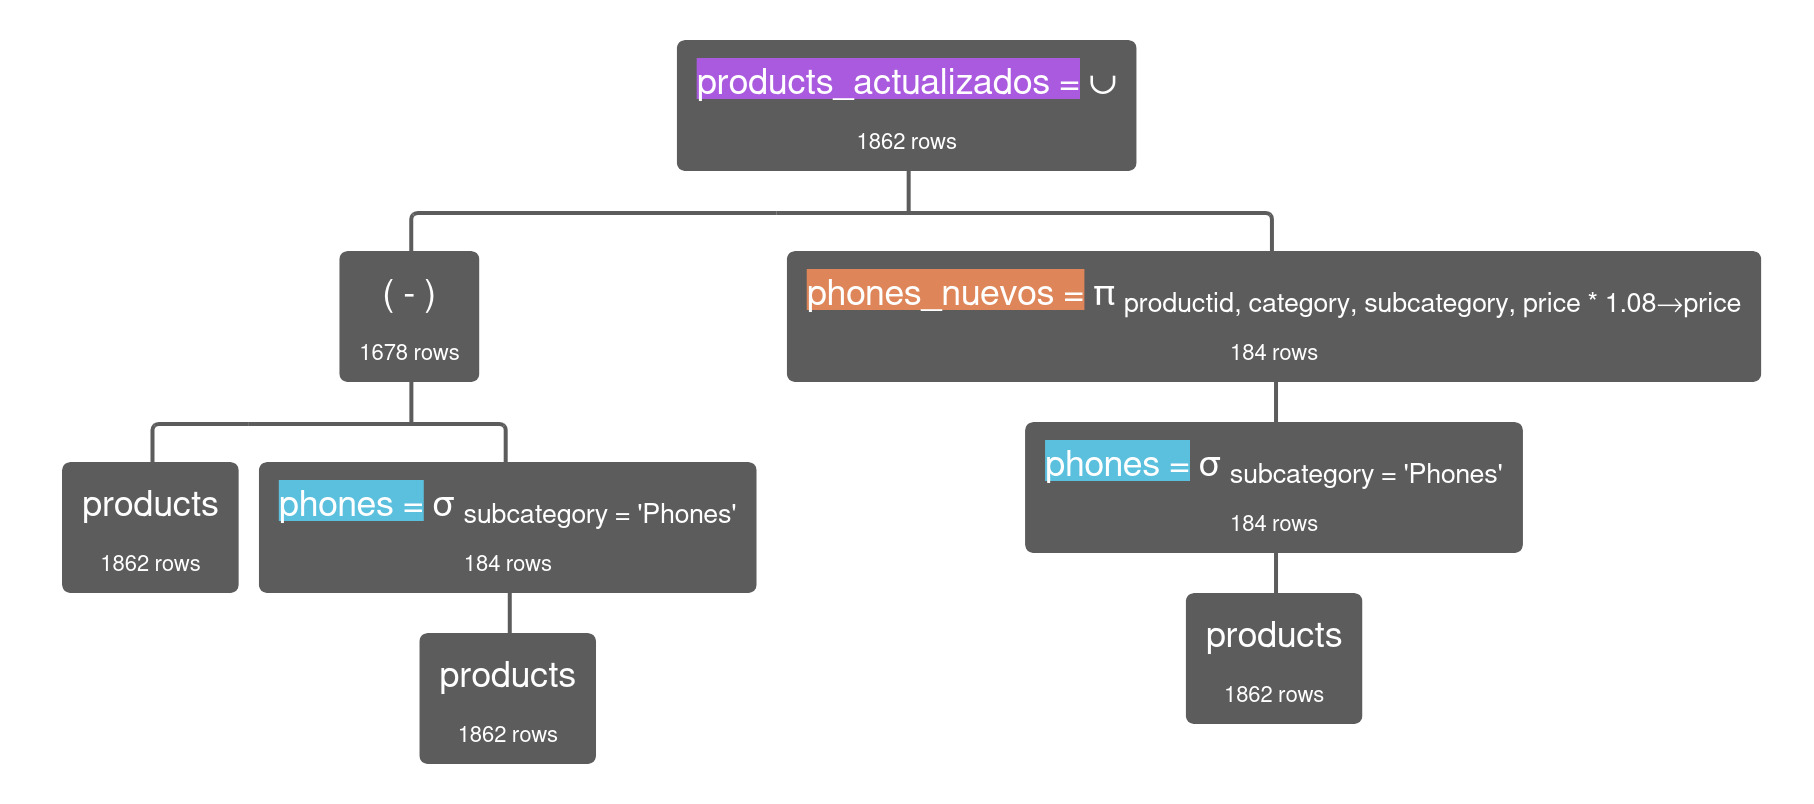
\includegraphics[width=0.72\textwidth]{figuras/3d_arbol.png}
\end{center}

\begin{center}
  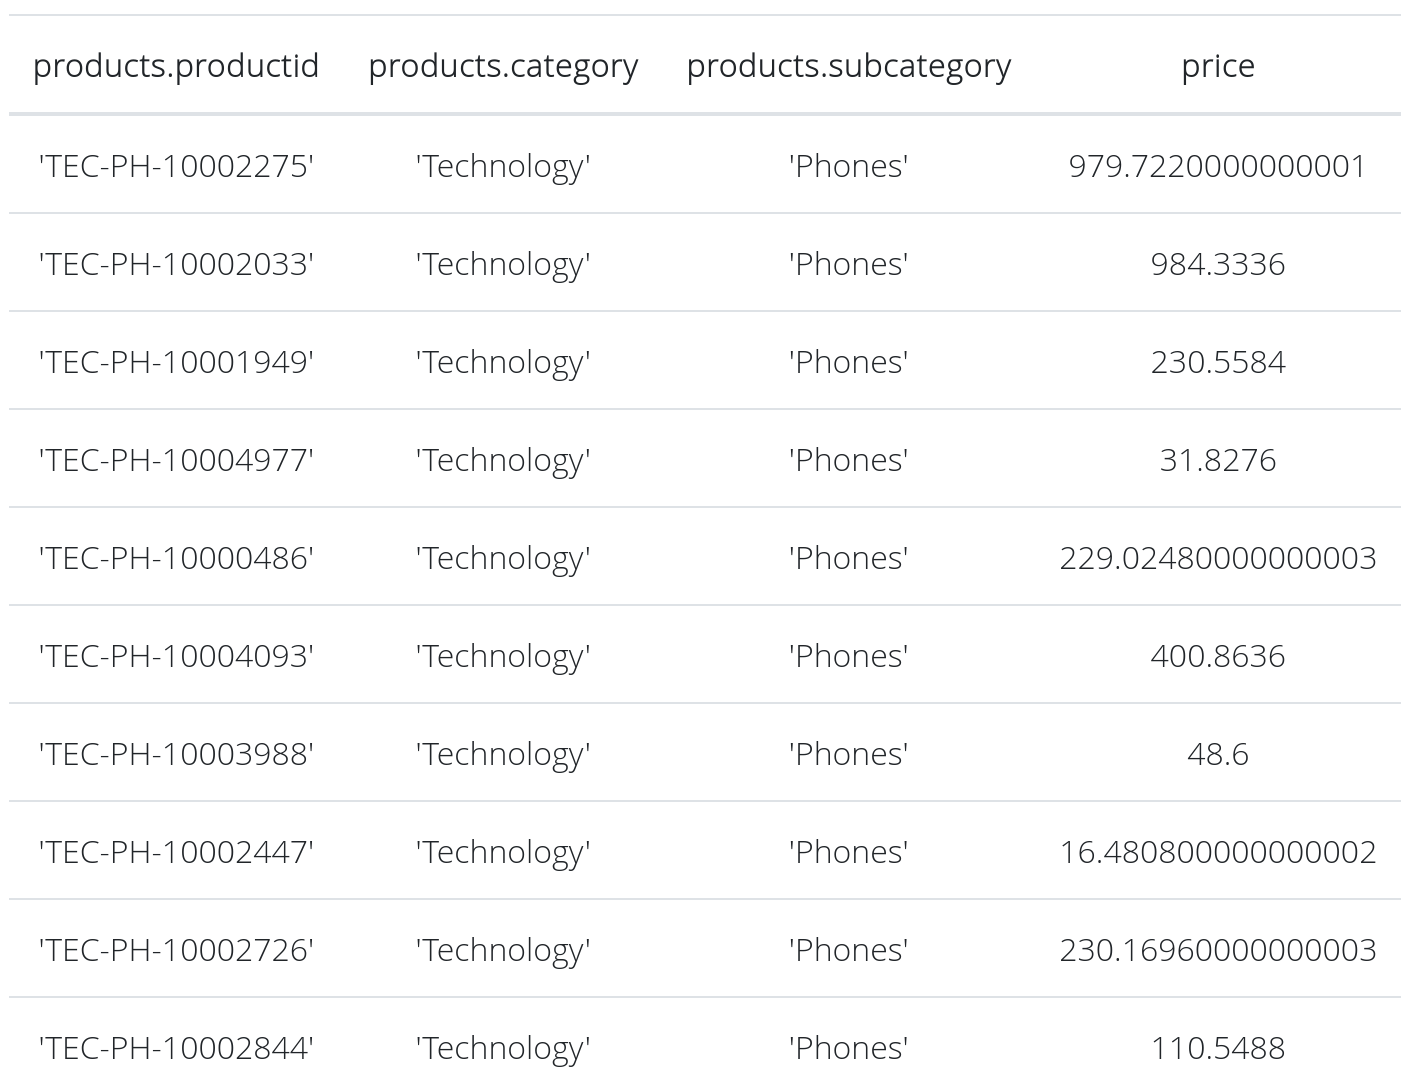
\includegraphics[width=0.55\textwidth]{figuras/3d_tuplas.png}
\end{center}

	% \newpage
\item Disminuir 8\% los precios de los productos de la categoría \textbf{Furniture} cuyo precio sea de \$600 a \$900. Aumentar en un 5\% los precios de la categoría \textbf{Technology} y subcategoría \textbf{Machines}.

\begin{lstlisting}
furn_en_rango = σ category = 'Furniture' ∧ price ≥ 600 ∧ price ≤ 900 (products)
tech_machines = σ category = 'Technology' ∧ subcategory = 'Machines' (products)

products = (products − furn_en_rango − tech_machines)
         ∪ π productid, category, subcategory, price * 0.92 → price (furn_en_rango)
         ∪ π productid, category, subcategory, price * 1.05 → price (tech_machines)
\end{lstlisting}

Se actualizan 13 productos de \texttt{Furniture} en el rango y 63 de
\texttt{Technology/Machines}; la relación \texttt{products} conserva sus
1862 renglones.

% ==========================================
% Página de mayor tamaño para el árbol y las tuplas
% (misma técnica que en la Práctica 05)
% ==========================================
\clearpage
\pdfpagewidth=35cm
\pdfpageheight=25cm
\setlength{\textwidth}{34cm}
\setlength{\hsize}{34cm}
\setlength{\oddsidemargin}{\dimexpr(\pdfpagewidth-\textwidth)/2 - 1in\relax}
\setlength{\evensidemargin}{\oddsidemargin}
\setlength{\textheight}{24cm}
\setlength{\vsize}{24cm}
\setlength{\headheight}{0pt}
\setlength{\headsep}{0pt}
\setlength{\topmargin}{\dimexpr(\pdfpageheight-\textheight)/2 - 1in\relax}
\thispagestyle{empty}
\vspace*{0.2cm}
\centering
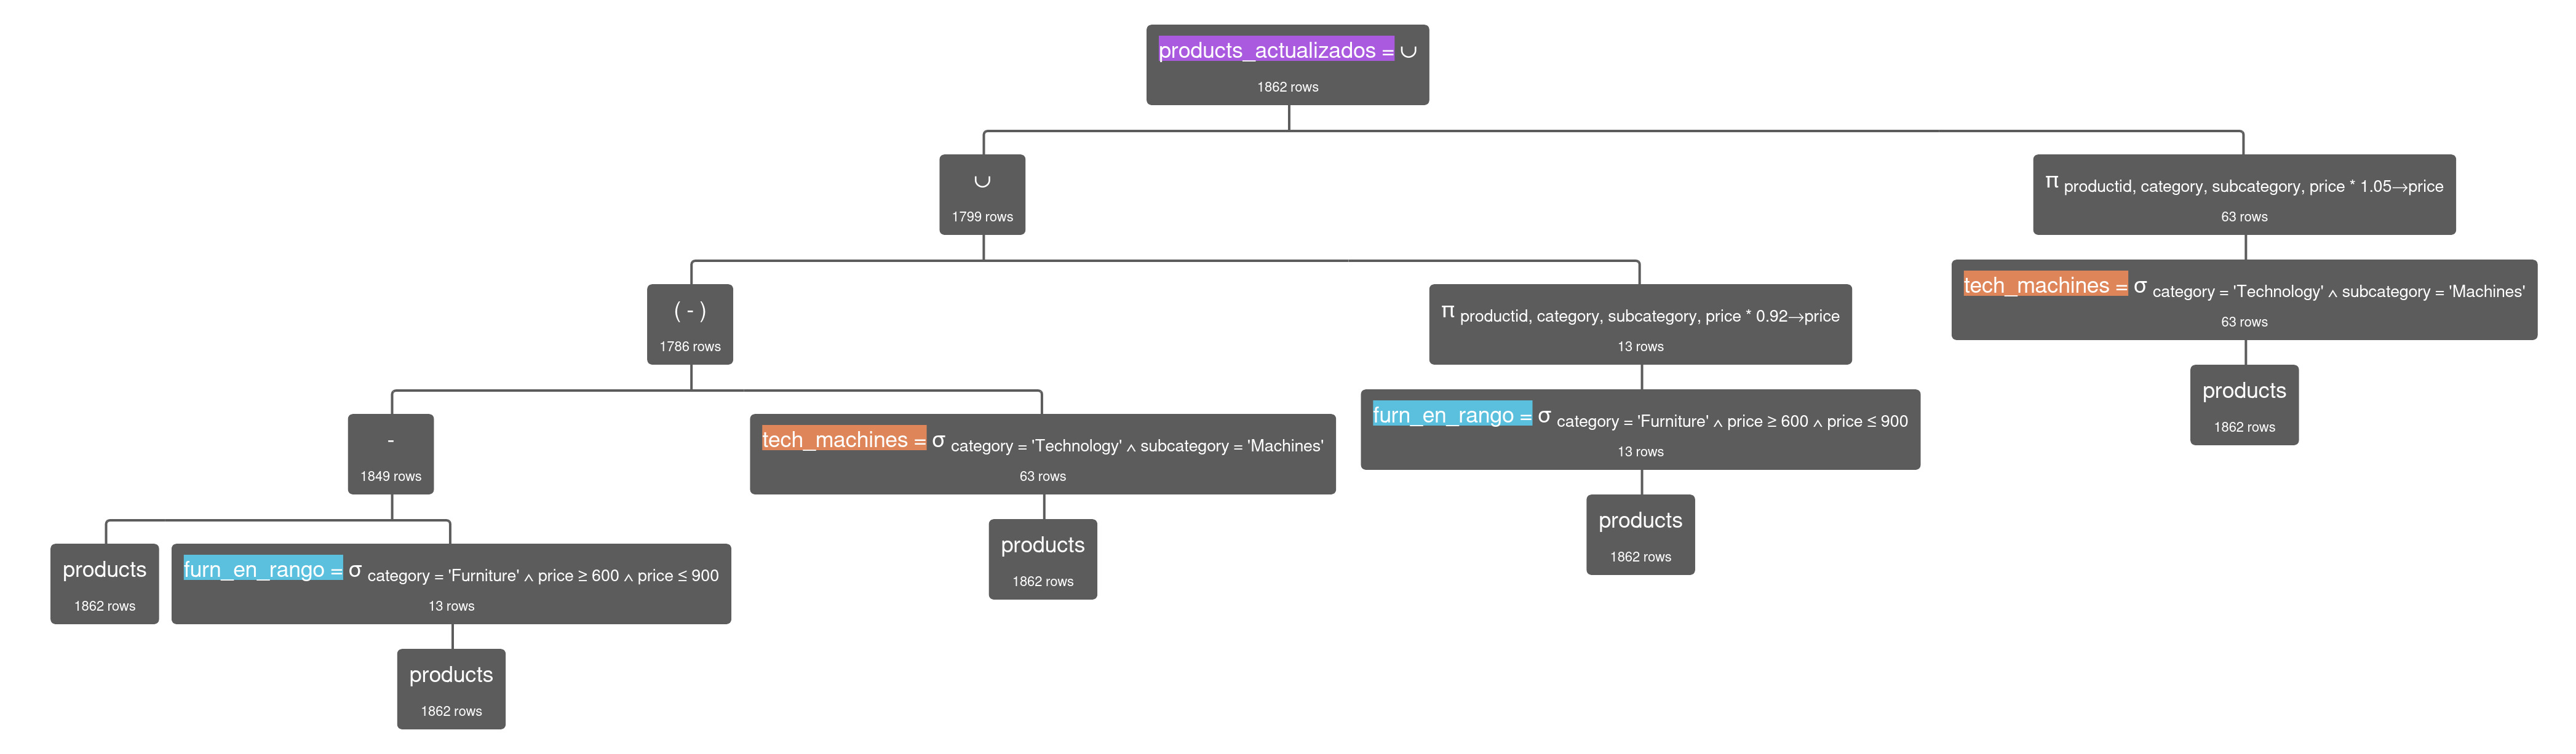
\includegraphics[width=\textwidth, height=0.38\textheight, keepaspectratio]{figuras/3e_arbol.png}

\vspace{0.35cm}
{\small Árbol de consulta de la actualización}

\vspace{0.45cm}
\begin{tabular}{@{}c@{\hspace{0.5cm}}c@{}}
\begin{minipage}[t]{0.38\textwidth}
  \centering
  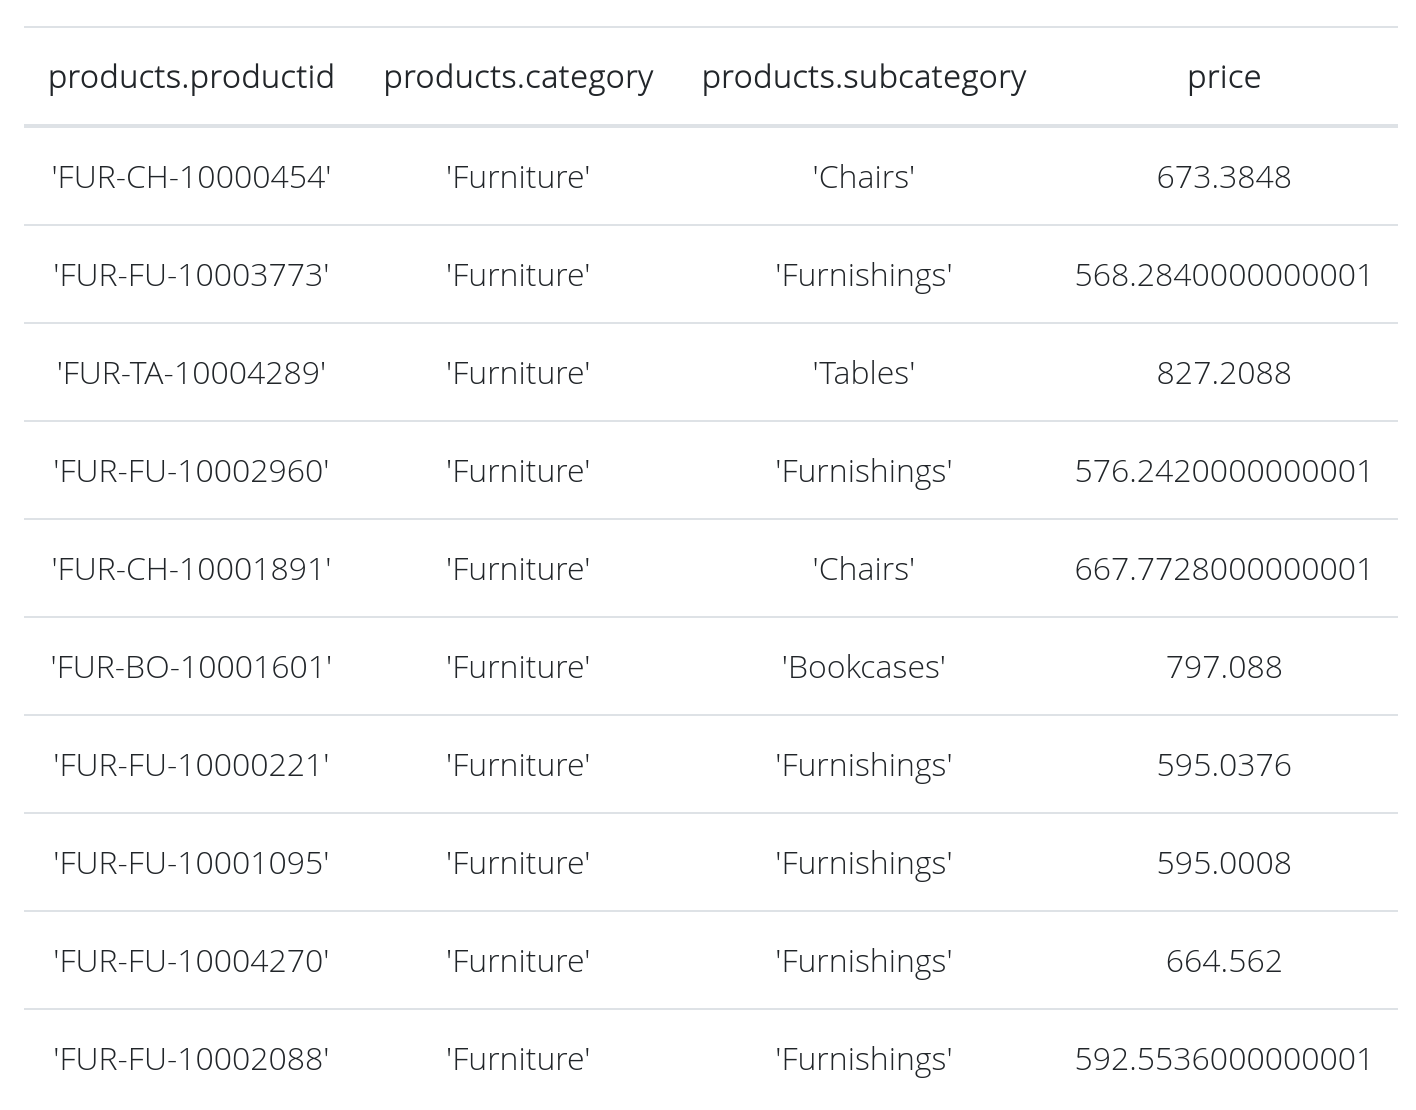
\includegraphics[width=\linewidth]{figuras/3e_tuplas_furn.png}\\[0.15cm]
  {\small Furniture actualizado}
\end{minipage} &
\begin{minipage}[t]{0.38\textwidth}
  \centering
  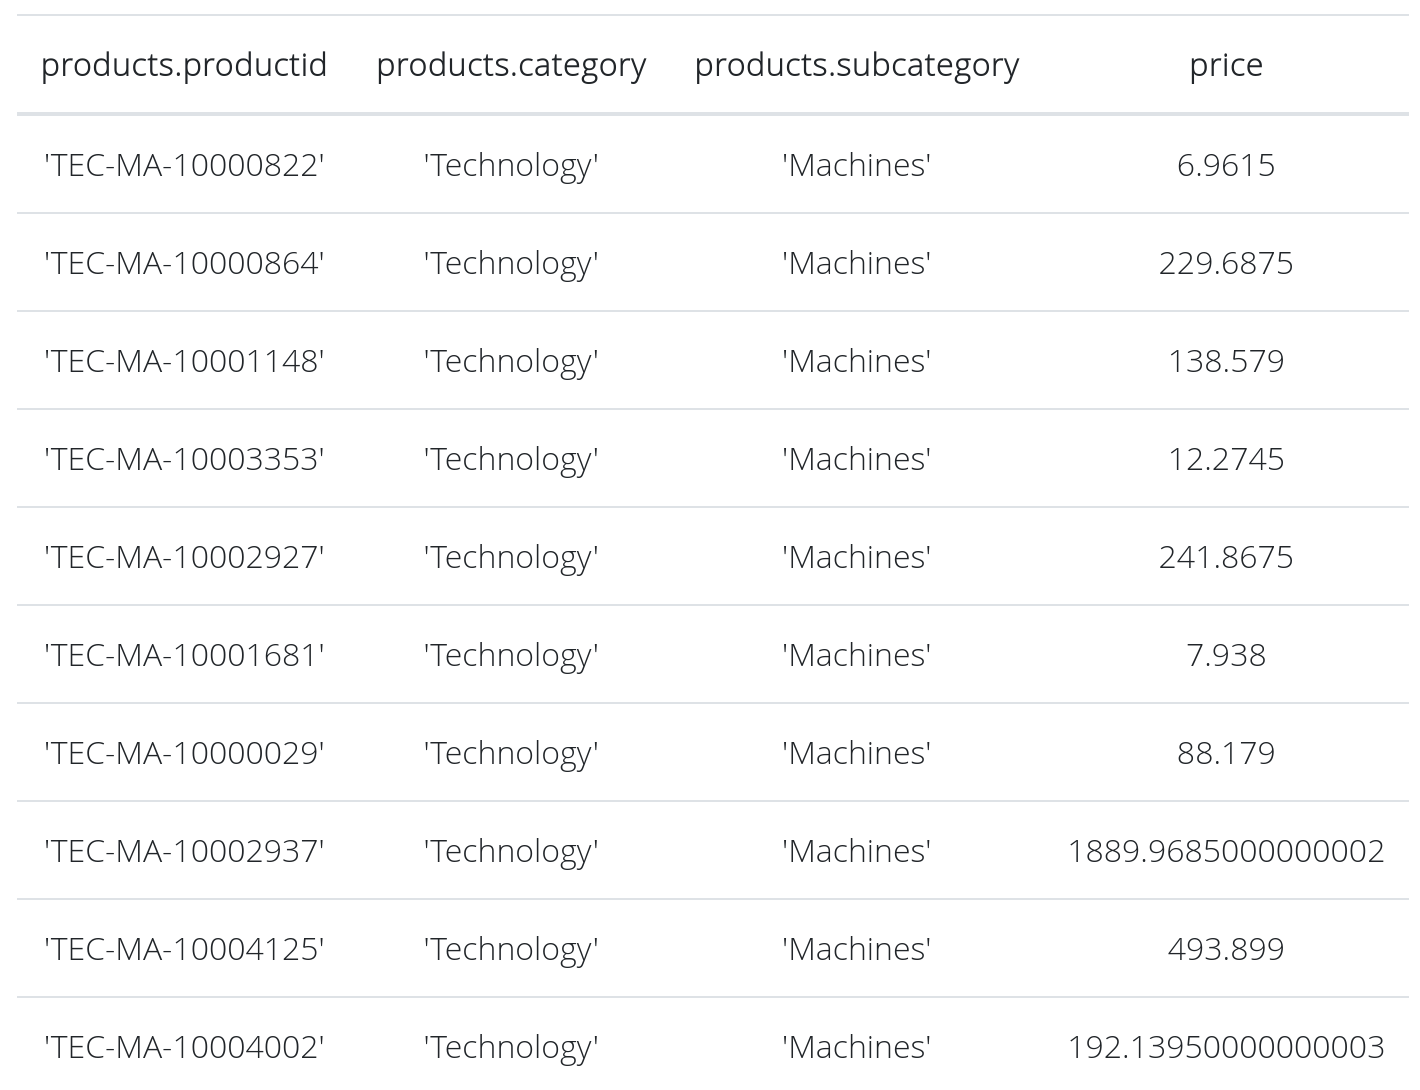
\includegraphics[width=\linewidth]{figuras/3e_tuplas_tech_machines.png}\\[0.15cm]
  {\small Technology/Machines actualizado}
\end{minipage}
\end{tabular}

\vspace{0.35cm}
{\small Las tuplas mostradas corresponden a los productos ya actualizados;
se presentan por separado porque en la tabla general de \texttt{products}
los 13 registros de \texttt{Furniture} y los 63 de
\texttt{Technology/Machines} son escasos entre 1862 renglones.}
\clearpage
\restoregeometry
\pdfpagewidth=\paperwidth
\pdfpageheight=\paperheight

\end{enumerate}

\printbibliography

\end{document}

